\documentclass[12pt,letterpaper]{article}

\usepackage[utf8]{inputenc}
\usepackage[T1]{fontenc}
\usepackage[spanish,es-tabla,es-nodecimaldot]{babel}
\usepackage[margin=1in]{geometry}
\usepackage{setspace}
\usepackage{fancyhdr}
\usepackage{enumitem}
\usepackage{amsmath}
\usepackage{amssymb}
\usepackage{graphicx}
\usepackage{tabularx}
\usepackage{array}
\usepackage{tikz}
\usetikzlibrary{arrows.meta,positioning,fit}
\usepackage{hyperref}
\usepackage{titlesec}

\hypersetup{colorlinks=true, linkcolor=black, urlcolor=black, citecolor=black,
            breaklinks=true}
\usepackage{url}
\Urlmuskip=0mu plus 1mu\relax
\makeatletter
\g@addto@macro{\UrlBreaks}{\UrlOrds}
\makeatother
\urlstyle{same}

\graphicspath{{../figuras/}}

\onehalfspacing

\pagestyle{fancy}
\fancyhf{}
\fancyhead[L]{\small Pulso - Predice, nutre, entrena y protege tu corazón}
\fancyhead[R]{\small\thepage}
\renewcommand{\headrulewidth}{0pt}

\titleformat{\section}{\normalfont\large\bfseries}{\thesection.}{0.6em}{\MakeUppercase}
\titleformat{\subsection}{\normalfont\normalsize\bfseries}{\thesubsection}{0.6em}{}

\setlist[itemize]{itemsep=4pt, topsep=6pt}
\setlist[enumerate]{itemsep=6pt, topsep=6pt}

% Tablas y figuras con el formato APA de la versión anterior (número en negrita,
% título en cursiva arriba, nota al pie en letra pequeña), numeradas solas.
\newcounter{tablaapa}
\newcounter{figuraapa}
\newcommand{\tablaAPA}[2]{\refstepcounter{tablaapa}\label{#1}%
  \noindent\textbf{Tabla \thetablaapa.} \textit{#2}\par\vspace{0.2cm}}
\newcommand{\figuraAPA}[2]{\refstepcounter{figuraapa}\label{#1}%
  \noindent\textbf{Figura \thefiguraapa.} \textit{#2}\par\vspace{0.2cm}}
\newcommand{\notaAPA}[1]{\par\vspace{0.15cm}\noindent\parbox{\linewidth}{\footnotesize\textit{Nota.} #1}\par}
\newcolumntype{L}{>{\raggedright\arraybackslash}X}
\newcolumntype{P}[1]{>{\raggedright\arraybackslash}p{#1}}
\newcolumntype{C}{>{\centering\arraybackslash}X}

\begin{document}

%======================= PORTADA =======================
\begin{titlepage}
\centering
\vspace*{1cm}

{\LARGE\bfseries Pulso - Predice, nutre, entrena y protege tu corazón\par}

\vspace{1.5cm}

{\large Plataforma PWA con IA para la Prevención Cardiovascular Global:\par}
\vspace{0.4cm}
{\large Predicción de Riesgo, Alimentación, Ejercicio y Seguimiento\par}
\vspace{0.4cm}
{\large Personalizado\par}

\vspace{2.5cm}

{\large Natalia Moncaleano Montero\par}
\vspace{0.4cm}
{\large Agustín Peralta Guarín\par}
\vspace{0.4cm}
{\large Diego Fernando Fandiño Olarte\par}

\vspace{2.5cm}

{\large Universidad de San Buenaventura\par}
\vspace{0.4cm}
{\large Facultad de Ingeniería (Bogotá)\par}
\vspace{0.4cm}
{\large Ingeniería de Sistemas\par}
\vspace{0.4cm}
{\large Bogotá D.C., Colombia\par}
\vspace{0.4cm}
{\large 2026\par}

\vfill
\end{titlepage}

\setcounter{page}{1}

%======================= DEDICATORIA =======================
\section*{DEDICATORIA}
\addcontentsline{toc}{section}{Dedicatoria}

Dedicamos este trabajo a nuestras familias, por su amor incondicional, comprensión
y apoyo constante durante todo el proceso de formación profesional. A nuestros
padres, quienes con su esfuerzo, valores y ejemplo nos impulsaron a superar cada
reto y alcanzar nuestras metas.

También dedicamos este logro a nuestros docentes, por compartir su conocimiento y
guiarnos con paciencia y compromiso, y a todas las personas que creyeron en
nosotros y nos motivaron a culminar con éxito este proyecto. Este trabajo es
reflejo del esfuerzo conjunto, la perseverancia y la pasión que compartimos como
grupo.

\newpage

%======================= INDICE =======================
\renewcommand{\contentsname}{ÍNDICE}
\tableofcontents

\newpage

%======================= RESUMEN =======================
\section*{RESUMEN}
\addcontentsline{toc}{section}{Resumen}

Las enfermedades cardiovasculares (ECV) constituyen la principal causa de muerte
en el mundo. De acuerdo con la Organización Mundial de la Salud (2026a), cada año
fallecen cerca de 20,5 millones de personas por esta causa, lo que equivale a una
de cada tres muertes registradas globalmente. La carga es desigual: los países de
ingresos medios y bajos concentran la mayor mortalidad evitable, en buena parte
porque sus poblaciones no acceden a herramientas de tamizaje y orientación
preventiva.

En ese contexto, este proyecto desarrolla \textbf{Pulso}, una Aplicación Web
Progresiva (PWA) de prevención cardiovascular que articula estimación de riesgo,
recomendaciones de alimentación, vida saludable y ejercicio, y seguimiento con
dashboard. Su núcleo técnico es un \textbf{motor de predicción propio},
implementado desde cero en TypeScript, sin librerías de aprendizaje automático ni
servicios de inteligencia artificial generativa, que integra tres componentes: el
pronóstico de las series temporales de cada usuario con ocho modelos, cuatro de
ellos benchmarks, seleccionados por backtesting según el error escalado MASE; un
índice de riesgo modificable de tipo log-lineal con coeficientes de meta-análisis
y atribución exacta por factor; y la detección de cambios sostenidos mediante
cartas CUSUM y EWMA. Un módulo de aprendizaje supervisado (regresión logística
por IRLS, gradient boosting y k vecinos más cercanos) permite entrenar y validar
el estimador con datos reales.

Sobre una cohorte sintética de 28 series con parámetros conocidos, el modelo que
el motor selecciona supera al pronóstico ingenuo en 23 de ellas, y CUSUM detecta
los cuatro cambios de régimen con un retraso medio de 4,5 días. Sobre 5.043
adultos de la Encuesta Nacional de Examen de Salud y Nutrición de los Estados
Unidos, ciclo 2021-2023 (Centers for Disease Control and Prevention [CDC], 2024),
con 11,8\,\% de antecedente cardiovascular y validación cruzada estratificada
5\,$\times$\,10, el índice del motor, sin entrenamiento, alcanza un área bajo la
curva ROC de 0,611 frente a 0,564 del puntaje heurístico previo, y una regresión
logística entrenada con las mismas variables no lo mejora (0,608). Al incorporar
edad y sexo, el índice llega a 0,799 y la regresión logística a 0,805, con
pendiente de calibración de 0,99; la diferencia entre ambos no es
estadísticamente significativa. Los coeficientes estimados coinciden con una
implementación independiente en numpy con diferencias del orden de $10^{-14}$. El
modelo de lenguaje se limita a redactar sobre los números que el motor calcula.

\vspace{0.4cm}
\noindent\textbf{Palabras clave:} enfermedades cardiovasculares, aprendizaje
automático, series temporales, regresión logística, validación cruzada,
estimación de riesgo, NHANES, PWA, salud digital.

\newpage

%======================= ABSTRACT =======================
\section*{ABSTRACT}
\addcontentsline{toc}{section}{Abstract}

\selectlanguage{english}

Cardiovascular diseases (CVDs) are the leading cause of death worldwide.
According to the World Health Organization (2026a), approximately 20.5 million
people die from CVDs every year, accounting for nearly one in every three
recorded deaths. The burden is unequally distributed: low- and middle-income
countries concentrate most of the preventable mortality, largely because their
populations lack access to screening tools and preventive guidance.

This work presents \textbf{Pulso}, a cardiovascular prevention Progressive Web
Application (PWA) that combines risk estimation, dietary, lifestyle and exercise
recommendations, and dashboard-based tracking. Its technical core is an
\textbf{in-house prediction engine}, implemented from scratch in TypeScript with
no machine learning libraries and no generative AI services, made of three
components: per-user time series forecasting with eight models, four of them
benchmarks, selected by backtesting on the scaled error MASE; a log-linear index
of modifiable risk with meta-analysis coefficients and exact per-factor
attribution; and detection of sustained changes with CUSUM and EWMA control
charts. A supervised learning module (logistic regression fitted by IRLS,
gradient boosting and k-nearest neighbours) makes it possible to train and
validate the estimator on real data.

On a synthetic cohort of 28 series with known parameters, the model selected by
the engine beats the naïve forecast in 23 of them, and CUSUM detects all four
regime changes with a mean delay of 4.5 days. On 5,043 adults from the United
States National Health and Nutrition Examination Survey, 2021-2023 cycle
(Centers for Disease Control and Prevention [CDC], 2024), with an 11.8\,\%
prevalence of cardiovascular history and 5\,$\times$\,10 stratified
cross-validation, the untrained engine index reaches an area under the ROC curve
of 0.611 against 0.564 for the previous heuristic score, and a logistic
regression trained on the same variables does not improve on it (0.608). When age
and sex are added, the index reaches 0.799 and the logistic regression 0.805,
with a calibration slope of 0.99; the difference between them is not
statistically significant. The estimated coefficients match an independent numpy
implementation with differences of the order of $10^{-14}$. The language model only writes text around
the figures computed by the engine.

\vspace{0.4cm}
\noindent\textbf{Keywords:} cardiovascular diseases, machine learning, time
series, logistic regression, cross-validation, risk estimation, NHANES, PWA,
digital health.

\selectlanguage{spanish}

\newpage

%======================= 1. INTRODUCCION =======================
\section{Introducción}

Las enfermedades cardiovasculares (ECV) son hoy uno de los problemas de salud
pública más serios a nivel global. La Organización Mundial de la Salud (2026a)
estima en 20,5 millones las muertes anuales por esta causa, cifra que equivale al
33\,\% de toda la mortalidad mundial y que viene en aumento sostenido año tras
año. En Colombia, el Ministerio de Salud y Protección Social (2022) reporta que
las enfermedades del sistema circulatorio son la primera causa de mortalidad
general, con una tasa ajustada superior a 130 muertes por cada 100.000
habitantes.

El panorama se complica por hábitos cada vez más extendidos: sedentarismo,
alimentación con exceso de sodio y grasas saturadas, tabaquismo, obesidad y altos
niveles de estrés. A esto se suma que muchas personas ignoran su nivel de riesgo
cardiovascular hasta que ocurre un evento agudo, típicamente un infarto o un
accidente cerebrovascular, lo que reduce drásticamente las posibilidades de
intervención preventiva.

Desde la ingeniería de sistemas existe una oportunidad concreta: construir un
sistema que recoja los indicadores de estilo de vida que una persona puede
registrar sin supervisión médica y los convierta en estimaciones de riesgo,
pronósticos y alertas verificables. La aplicación web progresiva (PWA) es el
medio de entrega elegido, porque ofrece la experiencia de una app nativa en
cualquier navegador sin pasar por tiendas de aplicaciones.

La literatura científica respalda el uso de aprendizaje automático en este
dominio. Weng et al. (2017) demostraron que los modelos de aprendizaje automático
pueden superar a los algoritmos clínicos clásicos en la predicción de eventos
cardiovasculares, y Krittanawong et al. (2020), en su meta-análisis, concluyen
que las redes neuronales profundas y los métodos de ensemble alcanzan exactitudes
superiores al 85\,\% a partir de datos clínicos estructurados. Esos desempeños se
obtienen sobre variables de laboratorio que una aplicación de uso abierto no
dispone, condición que delimita el alcance del presente trabajo y que se
cuantifica en la Sección~\ref{sec:resultados}.

Un riesgo frecuente en los prototipos de salud digital actuales es confundir la
integración de un modelo de lenguaje con capacidad predictiva. Un modelo
generativo puede redactar una recomendación convincente, pero no estima ni
valida nada, y cualquier proyección que escriba carece de respaldo numérico. Por
ello este trabajo separa las dos funciones: un motor de predicción propio,
auditable y evaluado contra benchmarks, calcula todas las cifras con su
incertidumbre y su procedencia, y el modelo de lenguaje se limita a redactar
sobre ellas.

Las Secciones~\ref{sec:motor}, \ref{sec:protocolo} y~\ref{sec:resultados}
describen el diseño del motor, los datos y el protocolo de evaluación, y los
resultados.

\newpage

%======================= 2. PLANTEAMIENTO =======================
\section{Planteamiento del Problema}

Las enfermedades cardiovasculares son hoy el principal desafío de salud pública
tanto a escala global como en Colombia. Según la OMS (2026a), causan cerca de
20,5 millones de muertes al año; las manifestaciones más frecuentes son
hipertensión arterial, cardiopatía isquémica y accidente cerebrovascular, todas
con tendencia ascendente en la última década.

Los factores de riesgo más prevalentes, sedentarismo, dietas con alto sodio y
grasas saturadas, tabaquismo, obesidad y estrés crónico, atraviesan economías de
todo nivel de ingreso. El problema operativo es que una gran parte de la
población no conoce su riesgo cardiovascular hasta que aparece un evento clínico,
porque no existen herramientas digitales gratuitas, accesibles y de alcance
masivo que permitan una evaluación preventiva personalizada (Weng et al., 2017).

Desde la ingeniería de sistemas se identifican dos brechas. La primera es de
acceso: las plataformas existentes suelen estar diseñadas para entornos
hospitalarios y dependen de exámenes de laboratorio, como la presión arterial o
el colesterol, que un usuario no aporta por su cuenta. La segunda es de rigor:
las herramientas de uso abierto suelen ofrecer puntajes heurísticos sin
evaluación y delegan la interpretación, e incluso la proyección del riesgo, en
modelos de lenguaje. El propio prototipo de Pulso partía de esa situación: un
puntaje calculado en el navegador sobre el último valor registrado de cada
indicador, con umbrales fijos, y una proyección redactada por el modelo de
lenguaje sin ningún cálculo que la respaldara.

\subsection*{Pregunta de Investigación}

A partir de lo anterior, la pregunta que orienta este trabajo es:

\begin{quote}
¿De qué manera una Aplicación Web Progresiva impulsada por inteligencia
artificial puede contribuir a la predicción, prevención y reducción del riesgo
cardiovascular a nivel mundial mediante recomendaciones personalizadas de
alimentación, ejercicio y vida saludable?
\end{quote}

Para que la respuesta sea verificable, la pregunta se descompone en cuatro
preguntas de ingeniería que la Sección~\ref{sec:resultados} responde con
mediciones:

\begin{enumerate}[label=P\arabic*.]
  \item ¿Los modelos de pronóstico ajustados sobre el historial de cada usuario
    superan a los benchmarks ingenuos, y con qué error?
  \item ¿Con qué retraso y con cuántas falsas alarmas se detecta un cambio
    sostenido en un indicador?
  \item ¿Cuánto discriminan, sobre datos poblacionales reales, los indicadores
    de estilo de vida que la aplicación captura, solos y junto con la edad y el
    sexo?
  \item ¿Un índice construido con coeficientes de la literatura, sin
    entrenamiento, rinde como un modelo entrenado con esos mismos datos?
\end{enumerate}

\subsection*{Antecedentes}

La aplicación de inteligencia artificial al área cardiovascular cuenta con
evidencia sólida. Weng et al. (2017) desarrollaron modelos de machine learning
que predicen eventos cardiovasculares con mayor precisión que SCORE o el
Framingham Risk Score. Krittanawong et al. (2020) confirman que las redes
neuronales profundas y los métodos de ensemble superan el 85\,\% de exactitud
sobre datos clínicos estructurados.

En prescripción de ejercicio, Liao et al. (2020) reportan que los sistemas de
recomendación basados en aprendizaje automático mejoran significativamente la
adherencia del paciente frente a planes genéricos. En nutrición computacional,
Zeevi et al. (2015) demostraron que modelos de IA pueden estimar respuestas
metabólicas individuales y proponer dietas ajustadas con resultados clínicamente
significativos.

En pronóstico de series temporales, la práctica recomendada es contrastar todo
modelo contra benchmarks simples, como repetir el último valor, la media o la
tendencia lineal entre extremos, y medir el error de forma escalada para poder
comparar series con unidades distintas; el MASE fue propuesto con ese fin
(Hyndman \& Koehler, 2006; Hyndman \& Athanasopoulos, 2021). En detección de
cambios, las cartas CUSUM (Page, 1954) y EWMA (Roberts, 1959) son el estándar
del control estadístico de procesos para desvíos pequeños y sostenidos
(Montgomery, 2019). En modelos de predicción clínica, la discriminación y la
calibración deben reportarse juntas, porque un modelo puede ordenar bien a las
personas y aun así asignarles probabilidades equivocadas (Van Calster et al.,
2019).

En cuanto a la arquitectura, Biduski et al. (2020) muestran que las PWA presentan
ventajas medibles sobre las apps nativas en contextos de salud pública: mejor
accesibilidad sin pasar por una store, funcionamiento offline para zonas con
conectividad intermitente, actualizaciones transparentes y un consumo de
almacenamiento marcadamente menor. En el caso colombiano, Pinzón et al. (2020) y
los informes del Observatorio Nacional de Salud (2021) han documentado barreras
estructurales como la falta de tamizaje digital para población general,
desigualdades regionales y baja adopción tecnológica en atención primaria.

\newpage

%======================= 3. JUSTIFICACION =======================
\section{Justificación}

\subsection{Relevancia Social}

Las enfermedades cardiovasculares son también, y sobre todo, un indicador de
desigualdad. Millones de personas en todo el mundo no cuentan con servicios de
salud preventivos, y eso eleva la mortalidad por eventos que podrían haberse
evitado. Pulso, como PWA gratuita y de alcance global, ayuda a reducir esa
brecha: pone al alcance de cualquiera una estimación orientativa de su riesgo, la
evolución proyectada de sus indicadores y una guía de hábitos adaptada a su
contexto, sin exigir exámenes de laboratorio.

La elección de la arquitectura PWA es estratégica para países de ingresos medios
y bajos, donde la conectividad es intermitente y la instalación desde una tienda
de aplicaciones es una barrera adicional.

\subsection{Relevancia Teórica}

El proyecto se apoya en una literatura ya establecida sobre IA aplicada a la
estratificación del riesgo (Weng et al., 2017; Krittanawong et al., 2020) y la
extiende en tres direcciones medibles. Primera, cuantifica sobre datos
poblacionales reales cuánto riesgo cardiovascular puede estimarse sin
laboratorio: los indicadores de estilo de vida discriminan de forma limitada por
sí solos (área bajo la curva ROC de 0,61), la edad y el sexo elevan esa cifra a
0,80, y aun así las variables de la aplicación aportan una mejora significativa
sobre el modelo que solo usa edad y sexo. Segunda, aporta evidencia de que un
índice construido con coeficientes de meta-análisis, sin entrenamiento, ordena a
las personas prácticamente igual que un modelo entrenado sobre los mismos datos,
lo que es relevante para cualquier herramienta preventiva que no dispone de
datos etiquetados propios. Tercera, traslada al seguimiento personal de salud dos
prácticas de otras disciplinas, la selección de modelos de pronóstico por
backtesting contra benchmarks y las cartas de control estadístico, y documenta
las decisiones que exigió adaptarlas a series cortas e irregulares.

\subsection{Relevancia Práctica}

Pulso permitirá a usuarios de cualquier país registrar sus indicadores de estilo
de vida y obtener, calculado por el motor y no por un modelo de lenguaje:

\begin{itemize}
  \item Un índice de riesgo modificable de 0 a 100, con los puntos que resta
    cada factor, la fuente bibliográfica de cada coeficiente y el multiplicador
    de contexto que aportan la edad y el sexo.
  \item El pronóstico a 30 días de cada indicador con intervalos de predicción
    del 80\,\% y el 95\,\%, el modelo que lo produjo y su error de backtesting.
  \item Alertas cuando un indicador cambia de forma sostenida, con la fecha
    estimada del cambio y su magnitud.
  \item La proyección del índice a 30 días, calculada sobre los pronósticos.
  \item Recomendaciones alimenticias, de vida saludable y de ejercicio
    redactadas a partir de esas cifras, con la instrucción explícita de no
    inventar números.
  \item Un dashboard con el historial, el pronóstico y la tabla de evaluación
    de los modelos, para que el usuario vea por qué el sistema dice lo que dice.
\end{itemize}

\newpage

%======================= 4. OBJETIVOS =======================
\section{Objetivos}

\subsection{Objetivo General}

Desarrollar Pulso, una Aplicación Web Progresiva (PWA) basada en inteligencia
artificial cuyo núcleo es un motor de predicción propio, entrenado y evaluado
contra benchmarks sobre datos reales y sintéticos, para la estimación del riesgo
cardiovascular, el pronóstico de los indicadores de estilo de vida y la
detección de cambios sostenidos, integrado con recomendaciones de alimentación,
vida saludable y ejercicio, y orientado a la prevención cardiovascular a nivel
mundial.

\subsection{Objetivos Específicos}

\begin{itemize}
  \item Diseñar la arquitectura de Pulso como PWA y, dentro de ella, un motor de
    predicción desacoplado de la interfaz y de los servicios de IA generativa,
    cuyos modelos, umbrales y coeficientes estén sustentados en la literatura y
    cuyas salidas incluyan siempre incertidumbre y procedencia.

  \item Implementar desde cero los componentes del motor: pronóstico de series
    temporales con selección por backtesting contra benchmarks, índice de riesgo
    modificable con atribución por factor, detección de cambios sostenidos y un
    módulo de aprendizaje supervisado; e integrarlos con los módulos funcionales
    de recomendaciones, rutinas y seguimiento.

  \item Entrenar y evaluar el estimador de riesgo sobre datos poblacionales
    reales con métricas de discriminación y calibración, validación cruzada
    estratificada repetida y comparación contra benchmarks; evaluar el
    pronóstico y la detección sobre cohortes sintéticas con parámetros
    conocidos; y verificar la implementación contra una referencia
    independiente.

  \item Validar el prototipo mediante pruebas de usabilidad con usuarios
    representativos, la revisión de un profesional de salud y la verificación
    del funcionamiento en distintos dispositivos y condiciones de conectividad.
\end{itemize}

\newpage

%======================= 5. ALCANCE Y LIMITACIONES =======================
\section{Alcance y Limitaciones}

\subsection{Alcance}

El proyecto contempla el desarrollo de Pulso como una PWA de alcance global,
basada en inteligencia artificial, orientada a la estimación del riesgo
cardiovascular, la generación de recomendaciones alimenticias con ingredientes
específicos, planes de vida saludable, rutinas de ejercicio personalizadas y el
seguimiento continuo del estado de salud del usuario. La plataforma estará
disponible para cualquier persona con navegador compatible, será instalable en
móvil, tablet o desktop, funcionará offline mediante Service Workers y enviará
notificaciones push para alertas preventivas. El sistema integra seis módulos
funcionales:

\begin{enumerate}
  \item Ingreso de indicadores de estilo de vida (frecuencia cardíaca en
    reposo, peso, horas de sueño y nivel de estrés) asociado a un identificador
    anónimo generado en el propio dispositivo, y un perfil opcional con edad,
    sexo, altura y tabaquismo, sin registro de usuario ni datos personales
    identificables.

  \item Motor de predicción, descrito en la Sección~\ref{sec:motor}: pronóstico
    de cada indicador, índice de riesgo modificable con atribución por factor,
    contexto de edad y sexo, proyección del índice y detección de cambios
    sostenidos. Reemplaza al puntaje heurístico de la versión inicial del
    prototipo y es la única fuente de las cifras que muestra la aplicación.

  \item Recomendaciones alimenticias personalizadas con ingredientes, cantidades,
    métodos de preparación, alternativas regionales y planes semanales con lista
    de compras automatizada.

  \item Recomendaciones de vida saludable que abarcan manejo del estrés, calidad
    del sueño, hidratación y hábitos cotidianos.

  \item Rutinas de ejercicio adaptadas al nivel de riesgo con progresividad
    automática y alertas de seguridad.

  \item Sistema de seguimiento con dashboard interactivo que muestra el
    historial, el pronóstico con sus intervalos, el modelo seleccionado y las
    alertas, y reportes periódicos exportables en PDF.
\end{enumerate}

\subsection{Limitaciones}

El proyecto presenta varias limitaciones que conviene declarar de entrada. El
desarrollo se limita a un prototipo funcional en fase experimental, sin
implementación directa en instituciones médicas. Las recomendaciones generadas
son de carácter orientativo y no sustituyen el criterio del profesional de
salud, y la exactitud de las estimaciones está condicionada por la calidad y
veracidad de los datos que ingrese el usuario, dado que el sistema no cuenta con
verificación clínica directa.

\textbf{El índice no es una escala clínica.} Sus coeficientes provienen de la
literatura, pero la combinación, la forma de las curvas entre los puntos citados
y la normalización son decisiones del proyecto. No estima probabilidades
absolutas de un evento y no reemplaza ecuaciones validadas como Framingham, que
requieren presión arterial y colesterol, variables que la aplicación no solicita
por decisión de diseño.

\textbf{Sobre los conjuntos de datos.} La fuente de entrenamiento y evaluación
del estimador es NHANES 2021-2023 (CDC, 2024), el único conjunto de acceso
público que mide las mismas variables que la aplicación captura. El UCI Heart
Disease (Janosi et al., 1988) es de acceso abierto y fue verificado: su
subconjunto usable, \texttt{processed.cleveland.data}, contiene 303 registros y
14 variables, de los cuales 6 presentan valores faltantes. Comparte con la
aplicación solo la edad y el sexo, y su frecuencia cardíaca es la máxima
alcanzada en prueba de esfuerzo, no la de reposo; por eso se usa para validar la
implementación de los algoritmos y no como fuente del estimador. El Framingham
Heart Study (Dawber et al., 1951) no es de descarga libre: su acceso se tramita
ante el repositorio BioLINCC del National Heart, Lung, and Blood Institute y
exige aprobación de un comité de ética y un acuerdo formal de uso de datos,
plazos incompatibles con el cronograma del trabajo. El Global Health Observatory
de la OMS (2026b) publica indicadores agregados por país y no registros
individuales, por lo que sustenta las cifras epidemiológicas de contexto pero no
permite entrenar un estimador individual.

\textbf{Restricciones de NHANES.} Condicionan la interpretación de la
Sección~\ref{sec:nhanes-resultados} y se declaran de manera explícita. Primera:
el diseño de la encuesta es transversal, de modo que el modelo estima la
asociación entre el estado actual del participante y el antecedente de un evento
cardiovascular, no la incidencia futura; el prototipo no realiza predicción
prospectiva de eventos. Segunda: el estrés se aproximó con el cuestionario PHQ-9
(Kroenke et al., 2001), que mide síntomas depresivos y no estrés percibido,
porque el ciclo no incluye una escala de estrés. Tercera: el desenlace es
autorreportado y no se verificó contra historia clínica. Cuarta: se omitieron
los ponderadores de muestreo complejo, lo que es admisible para evaluar un
clasificador pero impide generar estimaciones poblacionales. Quinta: NHANES
describe a la población de los Estados Unidos; la transferencia a población
colombiana requiere validación externa y recalibración, que queda planteada como
línea de trabajo posterior.

\textbf{Sobre la evaluación sintética.} Demuestra que la implementación es
correcta y describe su comportamiento frente a patrones conocidos, pero no mide
el desempeño sobre usuarios reales, para lo cual no existe todavía un historial
suficiente. Un conjunto público de series de dispositivos portátiles sería la
fuente natural para esa evaluación.

\newpage

%======================= 6. DISEÑO DEL MOTOR =======================
\section{Diseño del Motor de Predicción}
\label{sec:motor}

\subsection{Principios de Diseño}

El motor se construyó bajo cuatro reglas que se verifican en el código y en las
pruebas automatizadas:

\begin{itemize}
  \item \textbf{Pureza.} El módulo \texttt{src/lib/ml} no depende de la base de
    datos, de la interfaz ni del framework web. Se compila por separado y se
    ejecuta en segundos, lo que permite probarlo y evaluarlo sin levantar la
    aplicación.
  \item \textbf{Incertidumbre y procedencia en toda salida.} Cada pronóstico
    lleva intervalos del 80\,\% y el 95\,\%, y cada cifra del informe indica qué
    modelo la produjo, con qué error de backtesting y con qué nivel de confianza.
  \item \textbf{Los benchmarks compiten en igualdad.} Los modelos ingenuos
    implementan la misma interfaz que los demás y participan en la selección:
    un modelo más complejo solo se usa si gana en backtesting.
  \item \textbf{Degradación explícita.} Con pocos datos el motor lo declara
    (confianza baja, factor excluido, índice insuficiente) en lugar de
    extrapolar.
\end{itemize}

\subsection{Arquitectura}

La Figura~\ref{fig:arquitectura} resume el flujo. Los registros diarios se
convierten en una serie por indicador; sobre cada serie se seleccionan y ajustan
los modelos de pronóstico y se aplican las cartas de control; con los niveles
actuales y el perfil se calcula el índice, y con los pronósticos, su proyección.
El resultado es un informe serializable que consumen la interfaz y el modelo de
lenguaje. El entrenamiento y la evaluación se ejecutan fuera de línea, con
scripts reproducibles del mismo repositorio.

\begin{figure}[!htbp]
\figuraAPA{fig:arquitectura}{Arquitectura del motor de predicción y su integración con la aplicación}
\centering
\begin{tikzpicture}[
  caja/.style={draw=black!70, rounded corners=2pt, align=center, font=\footnotesize,
               text width=3.0cm, minimum height=1.1cm, inner sep=3pt, fill=white},
  motor/.style={caja, fill=black!7},
  flecha/.style={-{Stealth[length=1.8mm]}, black!75},
  punteada/.style={-{Stealth[length=1.8mm]}, black!55, dashed}]
  \node[caja]  (reg)   at (0, 0)       {Registros diarios\\[1pt]{\scriptsize FC, sueño, estrés, peso}};
  \node[motor] (serie) at (3.75, 0)    {Serie diaria\\[1pt]{\scriptsize grilla y nivel robusto}};
  \node[caja]  (perf)  at (3.75, -2.35){Perfil opcional\\[1pt]{\scriptsize edad, sexo, altura, tabaco}};
  \node[motor] (pron)  at (7.5, 1.65)  {Pronóstico\\[1pt]{\scriptsize 8 modelos y backtesting}};
  \node[motor] (camb)  at (7.5, 0)     {Cambios sostenidos\\[1pt]{\scriptsize CUSUM y EWMA}};
  \node[motor] (ind)   at (7.5, -1.65) {Índice de riesgo\\[1pt]{\scriptsize contexto y proyección}};
  \node[caja]  (inf)   at (11.25, 0)   {Informe\\[1pt]{\scriptsize cifras con procedencia}};
  \node[caja]  (ui)    at (9.7, -3.45) {Interfaz\\[1pt]{\scriptsize índice y dashboard}};
  \node[caja]  (llm)   at (12.8, -3.45){Modelo de lenguaje\\[1pt]{\scriptsize solo redacta}};
  \node[caja]  (off)   at (0, -3.45)   {Entrenamiento y evaluación\\[1pt]{\scriptsize fuera de línea}};
  \draw[flecha] (reg) -- (serie);
  \draw[flecha] (serie.east) -- (pron.west);
  \draw[flecha] (serie) -- (camb);
  \draw[flecha] (serie.east) -- (ind.west);
  \draw[flecha] (perf.east) -- (ind.west);
  \draw[flecha] (pron.east) -- (inf.west);
  \draw[flecha] (camb) -- (inf);
  \draw[flecha] (ind.east) -- (inf.west);
  \draw[flecha] (inf.south) -- (ui.north);
  \draw[flecha] (inf.south) -- (llm.north);
  \draw[punteada] (off.south) -- ++(0,-0.35) -| node[pos=0.25, below, font=\scriptsize] {valida modelos y coeficientes (NHANES, UCI, cohorte sintética)} (ind.south);
\end{tikzpicture}
\notaAPA{Las cajas sombreadas forman el motor (\texttt{src/lib/ml}). El pronóstico de
cada indicador alimenta también la proyección del índice. El modelo de lenguaje
recibe el informe ya calculado y no produce cifras. El entrenamiento y la
evaluación se ejecutan fuera de línea.}
\end{figure}

\subsection{Preparación de las Series}

Cada indicador se representa como una grilla diaria continua desde el primer
registro hasta la fecha actual; los días sin registro quedan vacíos, porque la
aplicación no obliga a registrar todos los días. La regresión lineal, Theil-Sen y
los benchmarks trabajan directamente sobre los días observados. Holt y
Holt-Winters exigen una grilla regular: para ellos se interpolan linealmente los
huecos interiores de hasta tres días, y si más del 40\,\% de los puntos serían
imputados, esos modelos no compiten en esa serie. El nivel actual de cada
indicador, que alimenta el índice, es la mediana de los últimos siete días, para
que una noche atípica no lo altere.

\subsection{Modelos de Pronóstico y Selección por Backtesting}

El motor ajusta los ocho modelos de la Tabla~\ref{tab:modelos}, todos con la misma
interfaz: ajustan sobre el historial y devuelven la media del pronóstico y su
desvío a cada horizonte $h$, con el que se construyen los intervalos del 80\,\% y
el 95\,\% (Hyndman \& Athanasopoulos, 2021). Los cuatro primeros son los
benchmarks. Theil-Sen (Theil, 1950; Sen, 1968) usa la mediana de las pendientes
entre todos los pares de puntos, de modo que un registro atípico no la desvía.
Holt (Holt, 2004) incorpora un parámetro de amortiguación $\phi$ (Gardner \&
McKenzie, 1985) para que la tendencia no se extrapole indefinidamente, y
Holt-Winters (Winters, 1960) agrega un patrón semanal. Los parámetros $\alpha$,
$\beta^*$ y $\phi$ se eligen por búsqueda en grilla minimizando el error a un paso.
Los cuantiles de la normal y de la $t$ de Student que definen los intervalos se
calculan con aproximaciones numéricas estándar (Abramowitz \& Stegun, 1964).

\begin{table}[!htbp]
\tablaAPA{tab:modelos}{Modelos de pronóstico implementados}
\small
\noindent\begin{tabularx}{\linewidth}{P{3.4cm}LLc}
\hline
\textbf{Modelo} & \textbf{Pronóstico a $h$ pasos} & \textbf{Desvío del error $\sigma_h$} & \textbf{$n$ mín.} \\
\hline
Naïve & $y_n$ & $\sigma\sqrt{h}$ & 2 \\
Media móvil ($k=7$) & media de los últimos $k$ registros & $\sigma\sqrt{1+1/k}$ & 3 \\
Drift & $y_n + h\,\frac{y_n-y_1}{t_n-t_1}$ & $\sigma\sqrt{h\,(1+h/(n-1))}$ & 3 \\
Naïve estacional ($m=7$) & mismo día de la semana anterior & $\sigma\sqrt{\lfloor (h-1)/m\rfloor+1}$ & 8 \\
Regresión lineal (OLS) & $a + b\,t_{n+h}$ & $s\sqrt{1+\frac{1}{n}+\frac{(t_{n+h}-\bar t)^2}{S_{tt}}}$, cuantil $t$ con $n-2$ gl & 5 \\
Theil-Sen & $\tilde a + \tilde b\,t_{n+h}$ & como OLS, con sus propios residuos & 5 \\
Holt amortiguado & $\ell_n + (\phi+\dots+\phi^h)\,b_n$ & $\sigma\sqrt{1+\sum_{j=1}^{h-1}(\alpha+\alpha\beta^*\phi_j)^2}$ & 10 \\
Holt-Winters aditivo ($m=7$) & $\ell_n + h\,b_n + s_{n+h-m(k+1)}$ & fórmula de Hyndman y Athanasopoulos (2021, \S\,8.7) & 21 \\
\hline
\end{tabularx}
\notaAPA{$\sigma$ es el desvío de los residuos a un paso; $\phi_j=\phi+\dots+\phi^j$;
$k=\lfloor (h-1)/m\rfloor$ en Holt-Winters. Los cuatro primeros modelos son los
benchmarks.}
\end{table}

\textbf{Backtesting.} Para cada serie se usa un esquema de origen móvil con
ventana expansiva: en cada día de origen $o$ con al menos 14 observaciones
previas, cada modelo se ajusta con lo observado antes de $o$ y pronostica los
siete días siguientes, que se comparan solo contra los días con registro real.
Nunca se usa validación cruzada aleatoria, porque mezclaría el futuro con el
pasado. La métrica de selección es el error absoluto escalado medio (Hyndman \&
Koehler, 2006):
\[
\mathrm{MASE}_o = \frac{\frac{1}{H}\sum_{h=1}^{H}\left|y_{o+h}-\hat y_{o+h}\right|}
{\frac{1}{o-1}\sum_{t=2}^{o}\left|y_t-y_{t-1}\right|},
\]
es decir, el error del modelo dividido por el error del pronóstico ingenuo dentro
del entrenamiento: un valor menor que 1 significa que el modelo supera a repetir
el último valor. Se reportan además MAE, RMSE y la cobertura empírica de los
intervalos, que en un intervalo honesto del 80\,\% debe rondar el 80\,\%.

\textbf{Selección.} Gana el menor MASE entre los modelos con al menos cinco
pronósticos evaluados; ante empate, el más simple. Con menos de 21 registros no
se compara y se usa la media móvil con confianza baja. La confianza es alta con
45 registros o más y MASE menor que 0,9, y media con 21 o más.

\subsection{Índice de Riesgo Modificable}

Para cada factor modificable $i$ con valor $x_i$, la función
$\ell_i(x_i)\geq 0$ es el logaritmo del riesgo relativo respecto de un rango de
referencia, en el que vale cero, y es continua, de modo que dormir cinco horas
pesa proporcionalmente más que dormir seis. Bajo el supuesto multiplicativo de
los modelos log-lineales, el índice combina los factores con datos así:
\[
L = \sum_i \ell_i(x_i), \qquad \mathrm{RR} = e^{L}, \qquad
L_{\max} = \sum_i \ell_i(x_i^{\mathrm{peor}}), \qquad
\mathrm{score} = 100\left(1 - \frac{L}{L_{\max}}\right).
\]
Como el puntaje es lineal en $L$, los puntos que resta cada factor son exactos y
aditivos, $100\,\ell_i/L_{\max}$, y la interfaz puede mostrarlos sin métodos de
atribución adicionales. La Tabla~\ref{tab:factores} presenta las funciones y sus
fuentes. Un factor sin datos se excluye de $L$ y de $L_{\max}$, y con menos de
dos factores el índice se declara insuficiente.

\begin{table}[!htbp]
\tablaAPA{tab:factores}{Factores del índice, funciones de log-riesgo relativo y fuentes}
\small
\noindent\begin{tabularx}{\linewidth}{P{1.9cm}P{2.15cm}LP{3.0cm}}
\hline
\textbf{Factor} & \textbf{Referencia} & \textbf{$\ell_i(x)$ fuera de la referencia} & \textbf{Fuente} \\
\hline
FC en reposo & 50--70 lpm & $\ln(1{,}09)\,\frac{\min(x,120)-70}{10}$ sobre 70; $\ln(1{,}10)\,\frac{50-\max(x,35)}{10}$ bajo 50 (evidencia débil) & Zhang et al. (2016); Aune et al. (2017) \\
Sueño & 7--8 h & $\frac{\ln 1{,}48}{2}\,(7-\max(x,3))$ bajo 7; $\frac{\ln 1{,}38}{2}\,(\min(x,12)-8)$ sobre 8 & Cappuccio et al. (2011); Yin et al. (2017) \\
Estrés (1--10) & hasta 3 & $\ln(1{,}27)\,\frac{\min(x,10)-3}{7}$ (evidencia débil: escala autorreportada) & Richardson et al. (2012) \\
IMC & 18,5--25 & $\ln(1{,}39)\,\frac{\min(x,40)-25}{5}$ sobre 25; $\ln(1{,}3)\,\frac{18{,}5-\max(x,15)}{3{,}5}$ bajo 18,5 (evidencia débil) & Global BMI Mortality Collaboration (2016) \\
Tabaquismo & no fuma & $\ln 2{,}5$ si fuma actualmente & Yusuf et al. (2004) \\
\hline
\end{tabularx}
\notaAPA{La curva de sueño está calibrada para valer $\ln 1{,}48$ con 5 horas y
$\ln 1{,}38$ con 10 horas, los riesgos relativos de sueño corto y largo del
meta-análisis citado.}
\end{table}

\textbf{Contexto no modificable.} La edad y el sexo no entran al puntaje, para
que refleje solo lo que la persona puede cambiar: alguien de 70 años con hábitos
excelentes no debe aparecer en riesgo por su edad. Se reportan aparte como un
multiplicador de contexto $e^{\ell_{\mathrm{edad}}+\ell_{\mathrm{sexo}}}$, con
$\ell_{\mathrm{edad}}=\frac{\ln 2}{10}(\min(e,90)-40)$ para edades mayores de 40
años, que expresa la duplicación aproximada del riesgo por década, y
$\ell_{\mathrm{sexo}}=\ln 1{,}5$ para el sexo masculino. La
Sección~\ref{sec:nhanes-resultados} contrasta ambos valores con los que aprende
un modelo entrenado.

\textbf{Proyección.} El mismo índice se evalúa sobre el pronóstico a 30 días de
cada indicador. Como las funciones tienen forma de U, el intervalo del puntaje
proyectado se obtiene evaluando todas las combinaciones de extremos de los
intervalos del 80\,\% ($2^k$ evaluaciones con $k\leq 4$). La proyección deja así
de ser un texto del modelo de lenguaje.

\subsection{Detección de Cambios Sostenidos}

Sobre cada indicador se estandariza $z_t=(y_t-\hat\mu)/\hat\sigma$ con una línea
base personal y se aplican dos cartas de control con los parámetros estándar de
Montgomery (2019):
\begin{gather*}
S^{+}_t=\max\!\left(0,\,S^{+}_{t-1}+z_t-k\right),\qquad
S^{-}_t=\max\!\left(0,\,S^{-}_{t-1}-z_t-k\right),\\
k=0{,}5,\qquad \text{alarma si } S^{\pm}_t>h=5;
\end{gather*}
\[
Z_t=\lambda y_t+(1-\lambda)Z_{t-1},\quad
\text{límites } \hat\mu \pm L\hat\sigma\sqrt{\tfrac{\lambda}{2-\lambda}\left(1-(1-\lambda)^{2t}\right)},\quad \lambda=0{,}2,\ L=3.
\]
CUSUM (Page, 1954) acumula desvíos pequeños y persistentes, como un aumento de
ocho latidos que se mantiene, que un umbral sobre valores individuales no
detecta; el día del cambio se estima como el último en que el acumulado valía
cero. EWMA (Roberts, 1959) funciona como verificación independiente. La
evaluación obligó a tres decisiones que no están en el manual. La línea base es
auto-iniciada (Hawkins, 1987): arranca con 14 observaciones y sigue incorporando
todas las siguientes, con media y varianza actualizadas por el método de
Welford (1962), hasta la primera alarma, cuando se congela; la primera versión,
con la base fija en 14 observaciones, disparaba 22 alarmas en 12 series estables.
Los valores estandarizados se winsorizan en $\pm 3$ para que un atípico aislado no
cargue la carta de una vez (Hawkins \& Olwell, 1998). Y las alarmas consecutivas
de un mismo desvío se consolidan en una sola alerta con fecha de inicio, de
detección y de última confirmación. Con menos de 15 registros no se emiten
alertas.

\subsection{Módulo de Aprendizaje Supervisado}

Para entrenar y validar el estimador con datos etiquetados se implementaron,
también desde cero y siguiendo la formulación de Hastie et al. (2009), los
siguientes componentes:

\begin{itemize}
  \item \textbf{Regresión logística} ajustada por mínimos cuadrados
    reponderados iterativamente (IRLS, método de Newton-Raphson), con una
    penalización ridge pequeña, $\lambda=0{,}01$, que garantiza que la hessiana
    sea invertible sin penalizar el intercepto (le Cessie \& van Houwelingen,
    1992). En cada iteración,
    \[
    \beta \leftarrow \beta + \left(X^{\top}WX+\lambda\tilde I\right)^{-1}
    \left(X^{\top}(y-p)-\lambda\tilde\beta\right),\qquad
    W=\mathrm{diag}\big(p_i(1-p_i)\big),
    \]
    y los errores estándar salen de la diagonal de la inversa de la hessiana en
    el óptimo. Las variables se estandarizan con los estadísticos de cada
    partición de entrenamiento, nunca con los de prueba.
  \item \textbf{Gradient boosting} con árboles de regresión (Friedman, 2001):
    parte del logaritmo de la odds de la prevalencia y en cada ronda ajusta un
    árbol de profundidad 3 al gradiente negativo de la log-verosimilitud, con un
    paso de Newton por hoja y tasa de aprendizaje $\nu=0{,}1$, durante 100 rondas.
  \item \textbf{k vecinos más cercanos} (Cover \& Hart, 1967) con distancia
    euclídea sobre variables estandarizadas, como comparador no paramétrico.
  \item \textbf{Métricas}: área bajo la curva ROC por el estadístico de
    Mann-Whitney (Hanley \& McNeil, 1982), puntaje de Brier, log-verosimilitud,
    diagrama de calibración, umbral de Youden (1950) y validación cruzada
    estratificada reproducible con semilla.
  \item \textbf{Lector del formato SAS Transport (XPORT) versión 5}, en el que el
    CDC publica los archivos de NHANES, con la conversión de los números en coma
    flotante IBM de base 16 y de los valores faltantes de SAS.
\end{itemize}

\subsection{Integración con la Aplicación y con el Modelo de Lenguaje}

El motor entra a la aplicación por un único punto: una acción de servidor que
carga 90 días de registros, el perfil y la adherencia a hábitos, y devuelve el
informe. La pantalla del índice muestra el puntaje, los puntos que resta cada
factor con su fuente, el contexto, la proyección con su intervalo y los cambios
detectados; el dashboard dibuja el pronóstico con sus bandas y la tabla de
backtesting del indicador seleccionado. Las tres rutas que usan un modelo de
lenguaje reciben únicamente el identificador del usuario; el servidor calcula el
informe y le entrega al modelo un resumen textual con todas las cifras y su
procedencia, con la instrucción de no inventar números ni proyecciones: ninguna
cifra que muestra la aplicación proviene de él.

\subsection{Verificación del Software}

El motor cuenta con 70 pruebas automatizadas, cada una contra un valor conocido y
no contra una salida guardada: por ejemplo, que el MASE del pronóstico ingenuo
dentro de la muestra valga exactamente 1, que Theil-Sen no se desvíe ante un
atípico que sí desvía a la regresión lineal, que CUSUM detecte un salto de tres
desvíos en pocas observaciones, que el gradient boosting aprenda una
interacción que la regresión logística no puede representar o que el lector
XPORT decodifique valores de coma flotante IBM conocidos. Además, la regresión
logística se reimplementó de forma independiente en numpy sobre los mismos datos
(Sección~\ref{sec:uci-resultados}). Todas las corridas usan semillas fijas y se
reproducen con los comandos del Anexo~A.

\newpage

%======================= 7. DATOS Y PROTOCOLO =======================
\section{Datos y Protocolo de Entrenamiento y Evaluación}
\label{sec:protocolo}

\subsection{Cohorte Sintética con Parámetros Conocidos}

No existe un historial real de usuarios con el cual evaluar el pronóstico y la
detección, y aunque existiera no se conocería el patrón verdadero contra el cual
medir. Por eso se generó una cohorte con parámetros conocidos y semilla fija:
para cada uno de los cuatro indicadores, siete perfiles de 90 días con rangos
fisiológicos y un 15\,\% de días sin registro, descritos en la
Tabla~\ref{tab:perfiles}, para un total de 28 series.

\begin{table}[!htbp]
\tablaAPA{tab:perfiles}{Perfiles de la cohorte sintética}
\small
\noindent\begin{tabularx}{\linewidth}{P{3.8cm}L}
\hline
\textbf{Perfil} & \textbf{Patrón generado} \\
\hline
Estable & Solo ruido alrededor de un nivel. \\
Tendencia suave y fuerte & Deriva lineal (por ejemplo, frecuencia cardíaca +0,05 y +0,15 lpm por día). \\
Estacional & Patrón semanal (por ejemplo, sueño +1,2 h los domingos y +0,9 h los sábados). \\
Cambio de régimen & Salto sostenido el día 45: frecuencia cardíaca +8 lpm, sueño $-1{,}2$ h, estrés +3, peso +2,5 kg. \\
Ruidoso & Desvío doble y 5\,\% de valores atípicos gruesos. \\
Disperso & 40\,\% de días sin registro y deriva suave. \\
\hline
\end{tabularx}
\end{table}

\subsection{Muestra Analítica de NHANES 2021-2023}

La muestra se construyó con siete archivos del ciclo agosto 2021 -- agosto 2023
(CDC, 2024), cruzados por identificador de participante y leídos con el lector
XPORT propio. La Tabla~\ref{tab:flujo} muestra el flujo de exclusiones y la
Tabla~\ref{tab:variables}, la correspondencia entre las variables de la
aplicación y las de la encuesta. El desenlace vale 1 si el participante respondió
afirmativamente a alguna de las cinco preguntas de antecedente cardiovascular y 0
si ninguna fue afirmativa y al menos una fue negativa. El resultado son
\textbf{5.043 adultos con 597 casos positivos (11,8\,\%)}, cuya caracterización
aparece en la Tabla~\ref{tab:descriptiva}.

\begin{table}[!htbp]
\tablaAPA{tab:flujo}{Flujo de construcción de la muestra analítica de NHANES 2021-2023}
\small
\noindent\begin{tabularx}{\linewidth}{Lr}
\hline
\textbf{Criterio} & \textbf{Participantes} \\
\hline
Participantes del ciclo (archivo demográfico) & 11.933 \\
Adultos de 18 años o más & 8.153 \\
Con pulso en reposo medido & 6.123 \\
Con peso e índice de masa corporal medidos & 6.061 \\
Con horas de sueño reportadas & 6.003 \\
Con los nueve ítems del PHQ-9 respondidos & 5.282 \\
Con desenlace cardiovascular conocido (muestra analítica) & 5.043 \\
\hline
\end{tabularx}
\end{table}

\begin{table}[!htbp]
\tablaAPA{tab:variables}{Correspondencia entre las variables de la aplicación y las de NHANES}
\small
\noindent\begin{tabularx}{\linewidth}{P{2.8cm}P{3.3cm}L}
\hline
\textbf{Aplicación} & \textbf{NHANES} & \textbf{Observación} \\
\hline
FC en reposo & \texttt{BPXOPLS1} & Pulso de la primera lectura oscilométrica, tras cinco minutos de reposo sentado. \\
Peso e IMC & \texttt{BMXWT}, \texttt{BMXBMI} & Medidos en el centro de examen, no autorreportados. En la aplicación el IMC sale del peso y de la altura del perfil. \\
Horas de sueño & \texttt{SLD012} & Horas de sueño en días laborables. \\
Estrés (1--10) & PHQ-9 (\texttt{DPQ010}--\texttt{DPQ090}) & Puntaje total de 0 a 27, llevado a la escala de la aplicación como $\mathrm{redondeo}(1+9\cdot\mathrm{PHQ}/27)$. Es una aproximación. \\
Tabaquismo & \texttt{SMQ020}, \texttt{SMQ040} & Fumador actual: al menos 100 cigarrillos en la vida y fuma todos o algunos días. Desconocido en 7 participantes, codificados como no fumadores. \\
Edad y sexo & \texttt{RIDAGEYR}, \texttt{RIAGENDR} & La encuesta agrupa en 80 las edades de 80 años o más. \\
Desenlace & \texttt{MCQ160B}--\texttt{MCQ160F} & Falla cardíaca, enfermedad coronaria, angina, infarto o accidente cerebrovascular, autorreportados. \\
\hline
\end{tabularx}
\end{table}

\begin{table}[!htbp]
\tablaAPA{tab:descriptiva}{Caracterización de la muestra analítica según el antecedente cardiovascular}
\small
\noindent\begin{tabularx}{\linewidth}{P{3.6cm}CCC}
\hline
\textbf{Variable} & \textbf{Total} \newline ($n=5.043$) & \textbf{Con antecedente} \newline ($n=597$) & \textbf{Sin antecedente} \newline ($n=4.446$) \\
\hline
Edad (años) & 53,6 $\pm$ 17,0 & 66,8 $\pm$ 10,8 & 51,8 $\pm$ 17,0 \\
Hombres & 45,4\,\% & 56,3\,\% & 43,9\,\% \\
FC en reposo (lpm) & 70,8 $\pm$ 12,3 & 70,8 $\pm$ 13,8 & 70,7 $\pm$ 12,0 \\
IMC (kg/m\textsuperscript{2}) & 29,7 $\pm$ 7,1 & 31,6 $\pm$ 7,6 & 29,5 $\pm$ 7,0 \\
Peso (kg) & 83,5 $\pm$ 21,8 & 88,5 $\pm$ 23,1 & 82,9 $\pm$ 21,6 \\
Sueño (h) & 7,7 $\pm$ 1,5 & 7,9 $\pm$ 1,9 & 7,6 $\pm$ 1,5 \\
PHQ-9 (0--27) & 4,0 $\pm$ 4,6 & 4,8 $\pm$ 5,0 & 3,9 $\pm$ 4,6 \\
Fumador actual & 14,5\,\% & 19,1\,\% & 13,8\,\% \\
\hline
\end{tabularx}
\notaAPA{Media $\pm$ desvío estándar; proporción en las variables binarias.}
\end{table}

\subsection{UCI Heart Disease}

El subconjunto Cleveland del UCI Heart Disease (Janosi et al., 1988; Detrano et
al., 1989) se usa para validar la implementación del módulo supervisado. Tras
descartar seis registros con faltantes quedan 297 pacientes derivados a
evaluación cardiológica, 137 de ellos con enfermedad coronaria (46,1\,\%), y
13 variables clínicas.

\subsection{Protocolo de Evaluación}

\textbf{Pronóstico y detección.} Para cada una de las 28 series sintéticas se
ejecuta la selección completa, es decir, el backtesting de los ocho modelos con
horizonte de siete días; se mide cuánto se acercan las pendientes estimadas a la
pendiente real y, en los perfiles con cambio de régimen, el retraso entre el
cambio verdadero y la primera alerta de cada carta. Las falsas alarmas se cuentan
en los perfiles estable y ruidoso.

\textbf{Estimador de riesgo.} Todos los modelos se evalúan sobre las mismas
particiones: validación cruzada estratificada de cinco particiones repetida diez
veces con semillas distintas, es decir, 50 evaluaciones fuera de muestra por
modelo, de las que se reportan media y desvío. Se comparan tres familias:
benchmarks (la prevalencia, que no discrimina, y una regresión logística con solo
edad y sexo); puntajes sin entrenamiento (el puntaje heurístico de la versión
inicial del prototipo, que asignaba 35, 35 y 30 puntos a frecuencia cardíaca,
sueño y estrés multiplicados por 1, 0,55 o 0,15 según su estado, y el índice del
motor, solo y combinado con su contexto de edad y sexo); y modelos entrenados
(regresión logística, gradient boosting y k vecinos, con $k=65\approx\sqrt{n}$ de
entrenamiento). Sobre las predicciones fuera de muestra de la primera repetición
se calculan la curva ROC, la calibración por deciles, el umbral de Youden y las
diferencias de área bajo la curva entre pares de modelos, con intervalos de
confianza del 95\,\% por bootstrap pareado de 2.000 remuestreos (Efron \&
Tibshirani, 1993). Los hiperparámetros de gradient boosting y de k vecinos no se
optimizaron: se usan como comparadores con valores estándar.

\textbf{Implementación.} En UCI se repite el mismo protocolo de validación
cruzada con tres conjuntos de variables, y los coeficientes de la regresión
logística ajustada a toda la muestra, tanto en UCI como en NHANES, se comparan
con los de la implementación independiente en numpy.

\newpage

%======================= 8. RESULTADOS =======================
\section{Resultados}
\label{sec:resultados}

\subsection{Pronóstico Frente a Benchmarks}

La Tabla~\ref{tab:mase} resume el backtesting sobre las 28 series. El modelo que
el motor selecciona supera al pronóstico ingenuo (MASE menor que 1) en
\textbf{23 de las 28 series}, y en 20 de ellas el elegido no es un benchmark. Las
series restantes son aquellas en las que el ruido domina y un benchmark es,
honestamente, lo mejor disponible; el motor lo reconoce en lugar de forzar un
modelo complejo. La media móvil es un benchmark exigente: su MASE medio iguala al
de la regresión lineal y al de Theil-Sen, y gana en 8 series, entre ellas las
tres estables de frecuencia cardíaca, sueño y peso. La cobertura empírica media de
los intervalos del 80\,\% está entre el 74\,\% y el 81\,\% en los modelos que no
son el naïve ni el drift; esos dos cubren el 93\,\%, es decir, sus intervalos son
demasiado anchos, una de las razones por las que pierden.

\begin{table}[!htbp]
\tablaAPA{tab:mase}{Desempeño de los modelos de pronóstico en la cohorte sintética}
\small
\noindent\begin{tabularx}{\linewidth}{P{5.4cm}CCCC}
\hline
\textbf{Modelo} & \textbf{MASE medio} & \textbf{MASE mediana} & \textbf{Cobertura IC 80\,\%} & \textbf{Series ganadas} \\
\hline
Naïve (benchmark) & 1,11 & 1,10 & 93\,\% & 0 \\
Media móvil de 7 días (benchmark) & 0,88 & 0,87 & 81\,\% & 8 \\
Drift (benchmark) & 1,17 & 1,13 & 93\,\% & 0 \\
Naïve estacional (benchmark) & 1,11 & 1,07 & 78\,\% & 0 \\
Regresión lineal (OLS) & 0,88 & 0,86 & 78\,\% & 8 \\
Theil-Sen & 0,88 & 0,86 & 78\,\% & 6 \\
Holt amortiguado & 0,90 & 0,87 & 74\,\% & 5 \\
Holt-Winters semanal & 1,04 & 1,01 & 80\,\% & 1 \\
\hline
\end{tabularx}
\notaAPA{Backtesting de origen móvil con horizonte de 7 días, semilla 42. Holt y
Holt-Winters compiten en 27 series porque en una serie dispersa la fracción
imputada supera el 40\,\%.}
\end{table}

\begin{figure}[!htbp]
\figuraAPA{fig:mase}{Error de pronóstico por modelo relativo al pronóstico ingenuo}
\centering
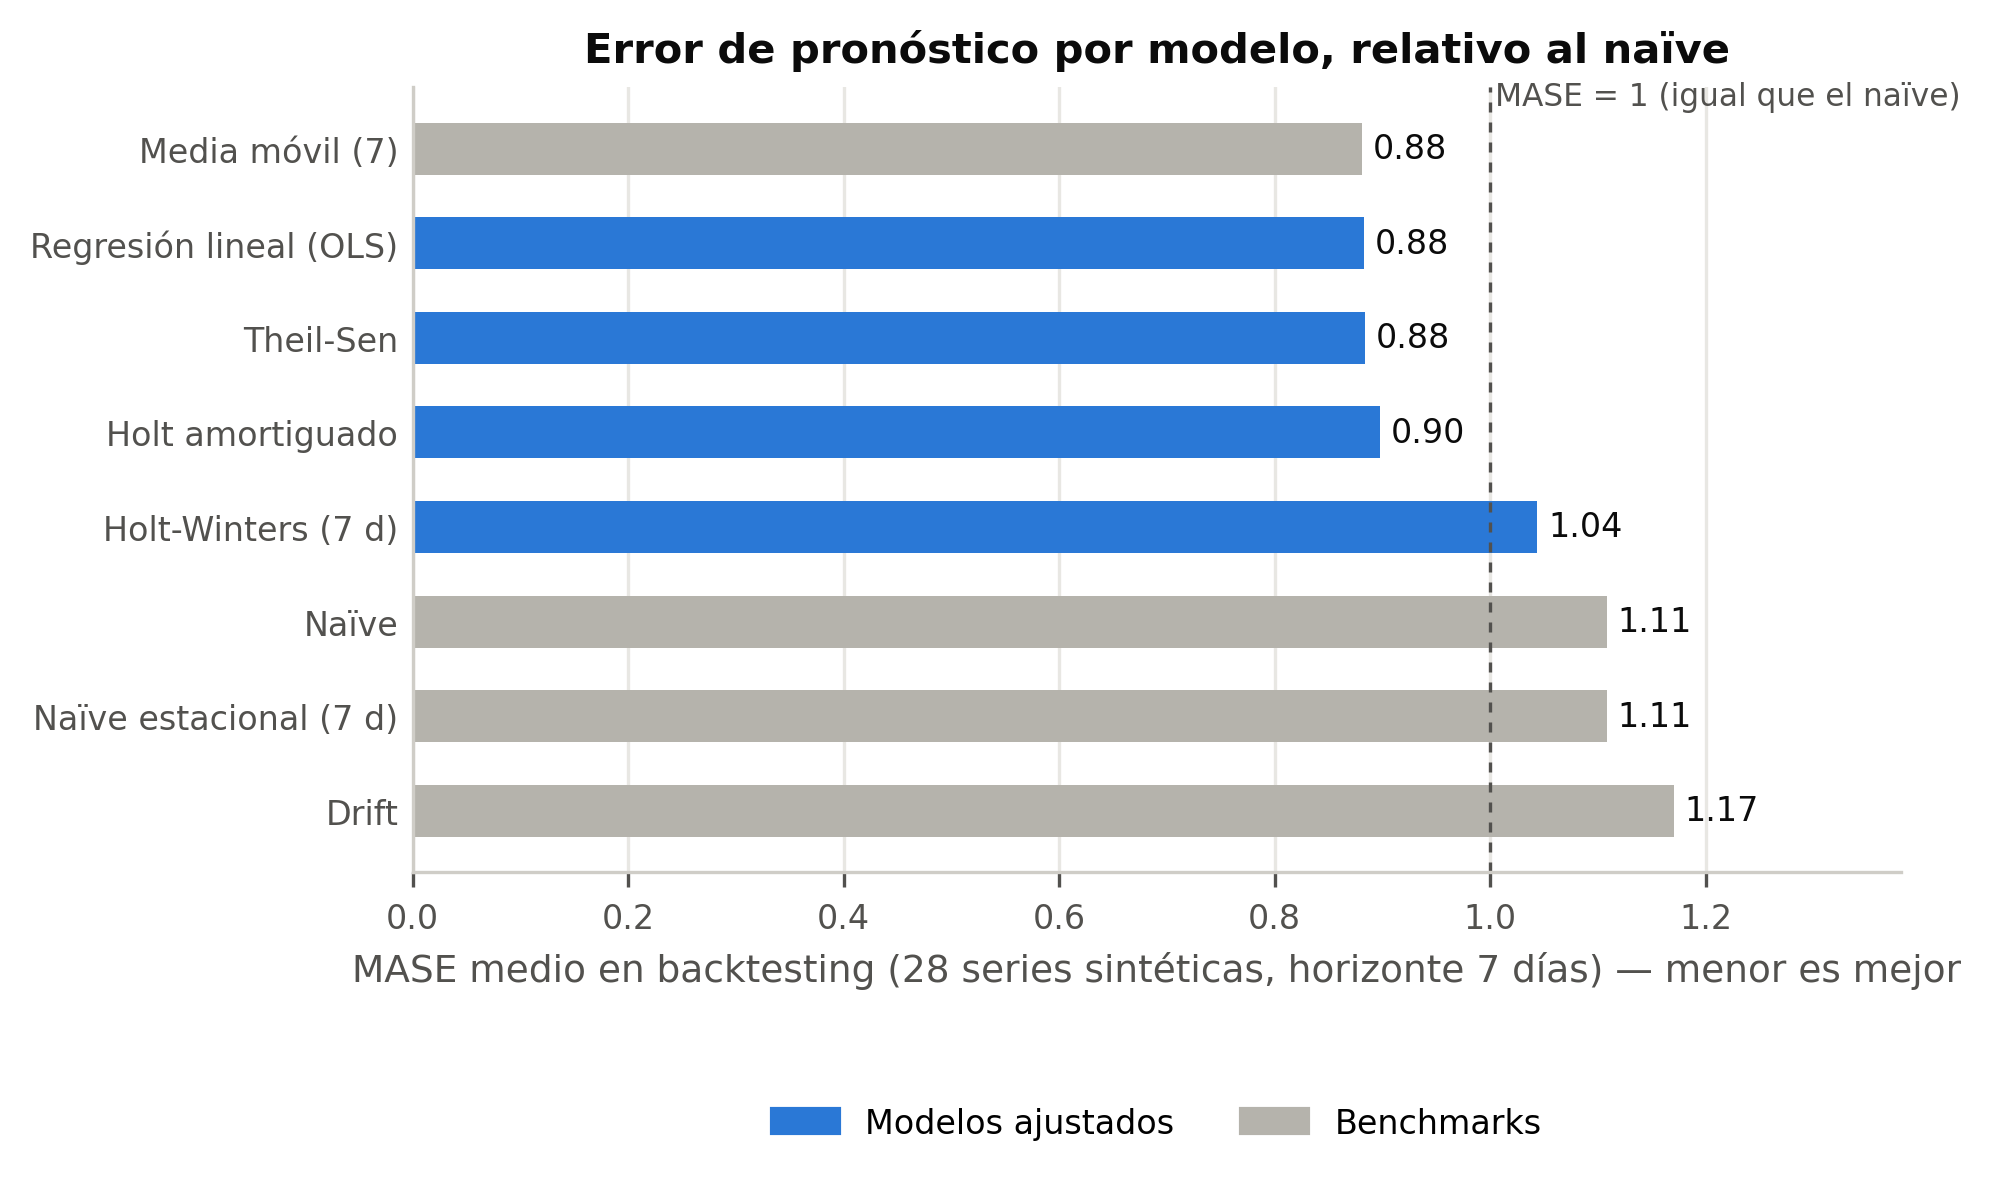
\includegraphics[width=0.86\linewidth]{fig1-mase-por-modelo.png}
\notaAPA{MASE medio en las 28 series; los benchmarks aparecen en gris. La línea
discontinua marca MASE $=1$.}
\end{figure}

Los modelos también recuperan los parámetros verdaderos. En las series con
tendencia, la regresión lineal y Theil-Sen estiman la pendiente real con un error
del orden del ruido: en peso con tendencia fuerte, la pendiente real de
$-0{,}080$ kg por día se estima en $-0{,}080$ con ambos métodos, y en frecuencia
cardíaca con tendencia fuerte, la real de 0,150 lpm por día se estima en 0,160 y
0,167. Holt-Winters recupera la amplitud semanal verdadera, por ejemplo 1,76
horas frente a 1,60 en sueño y 2,23 frente a 2,30 en estrés
(Figura~\ref{fig:pendientes}).

\begin{figure}[!htbp]
\figuraAPA{fig:pendientes}{Pendiente estimada frente a pendiente real en las series con tendencia}
\centering
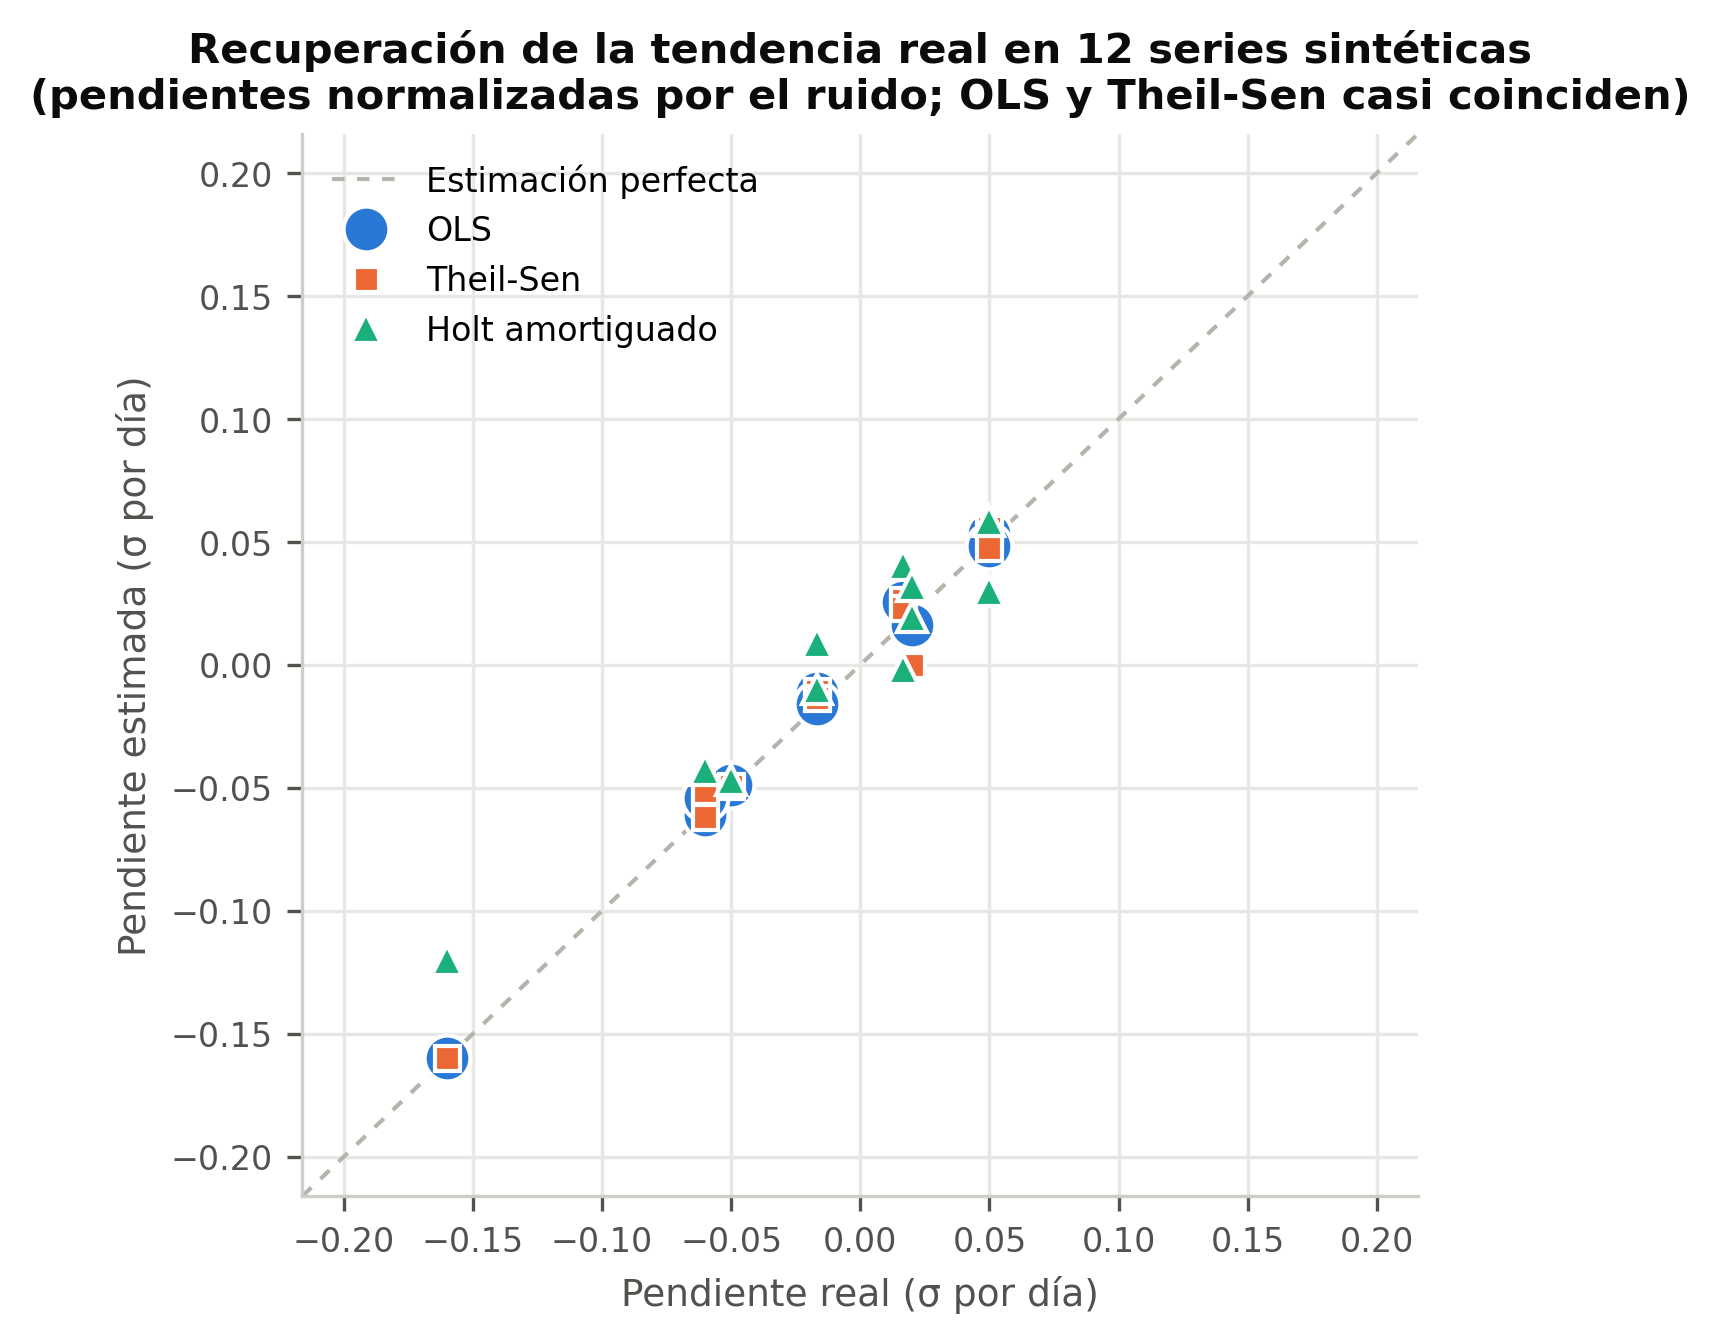
\includegraphics[width=0.56\linewidth]{fig7-pendientes-recuperadas.png}
\notaAPA{Pendientes normalizadas por el desvío del ruido de cada serie. La
diagonal representa la estimación perfecta.}
\end{figure}

\subsection{Detección de Cambios Sostenidos}

Las dos cartas detectan los cuatro cambios de régimen
(Tabla~\ref{tab:deteccion}): CUSUM con un retraso medio de \textbf{4,5 días} y
EWMA de 5,8 días. En los perfiles estable y ruidoso se registraron 5 falsas
alarmas en 8 series de 90 días, 0,6 por serie, y el perfil ruidoso incluye a
propósito atípicos de $\pm 5$ desvíos. Las series con tendencia también disparan
alertas, lo que es correcto: una deriva sostenida es un cambio de régimen. Las
cartas no modelan el patrón semanal; en los cuatro perfiles estacionales no hubo
alertas, pero un fin de semana muy distinto del resto podría dispararlas, y esa
limitación se declara. La Figura~\ref{fig:cusum} ilustra el funcionamiento de
CUSUM sobre una serie con un salto conocido.

\begin{table}[!htbp]
\tablaAPA{tab:deteccion}{Retraso de detección del cambio de régimen por indicador}
\small
\noindent\begin{tabularx}{\linewidth}{P{4.4cm}CCC}
\hline
\textbf{Indicador} & \textbf{Salto introducido} & \textbf{Retraso CUSUM} & \textbf{Retraso EWMA} \\
\hline
Frecuencia cardíaca & +8 lpm & 5 días & 5 días \\
Horas de sueño & $-1{,}2$ h & 9 días & 12 días \\
Nivel de estrés & +3 puntos & 2 días & 4 días \\
Peso & +2,5 kg & 2 días & 2 días \\
\hline
Media & & 4,5 días & 5,8 días \\
\hline
\end{tabularx}
\end{table}

\begin{figure}[!htbp]
\figuraAPA{fig:cusum}{Detección de un desvío sostenido de la frecuencia cardíaca con CUSUM}
\centering
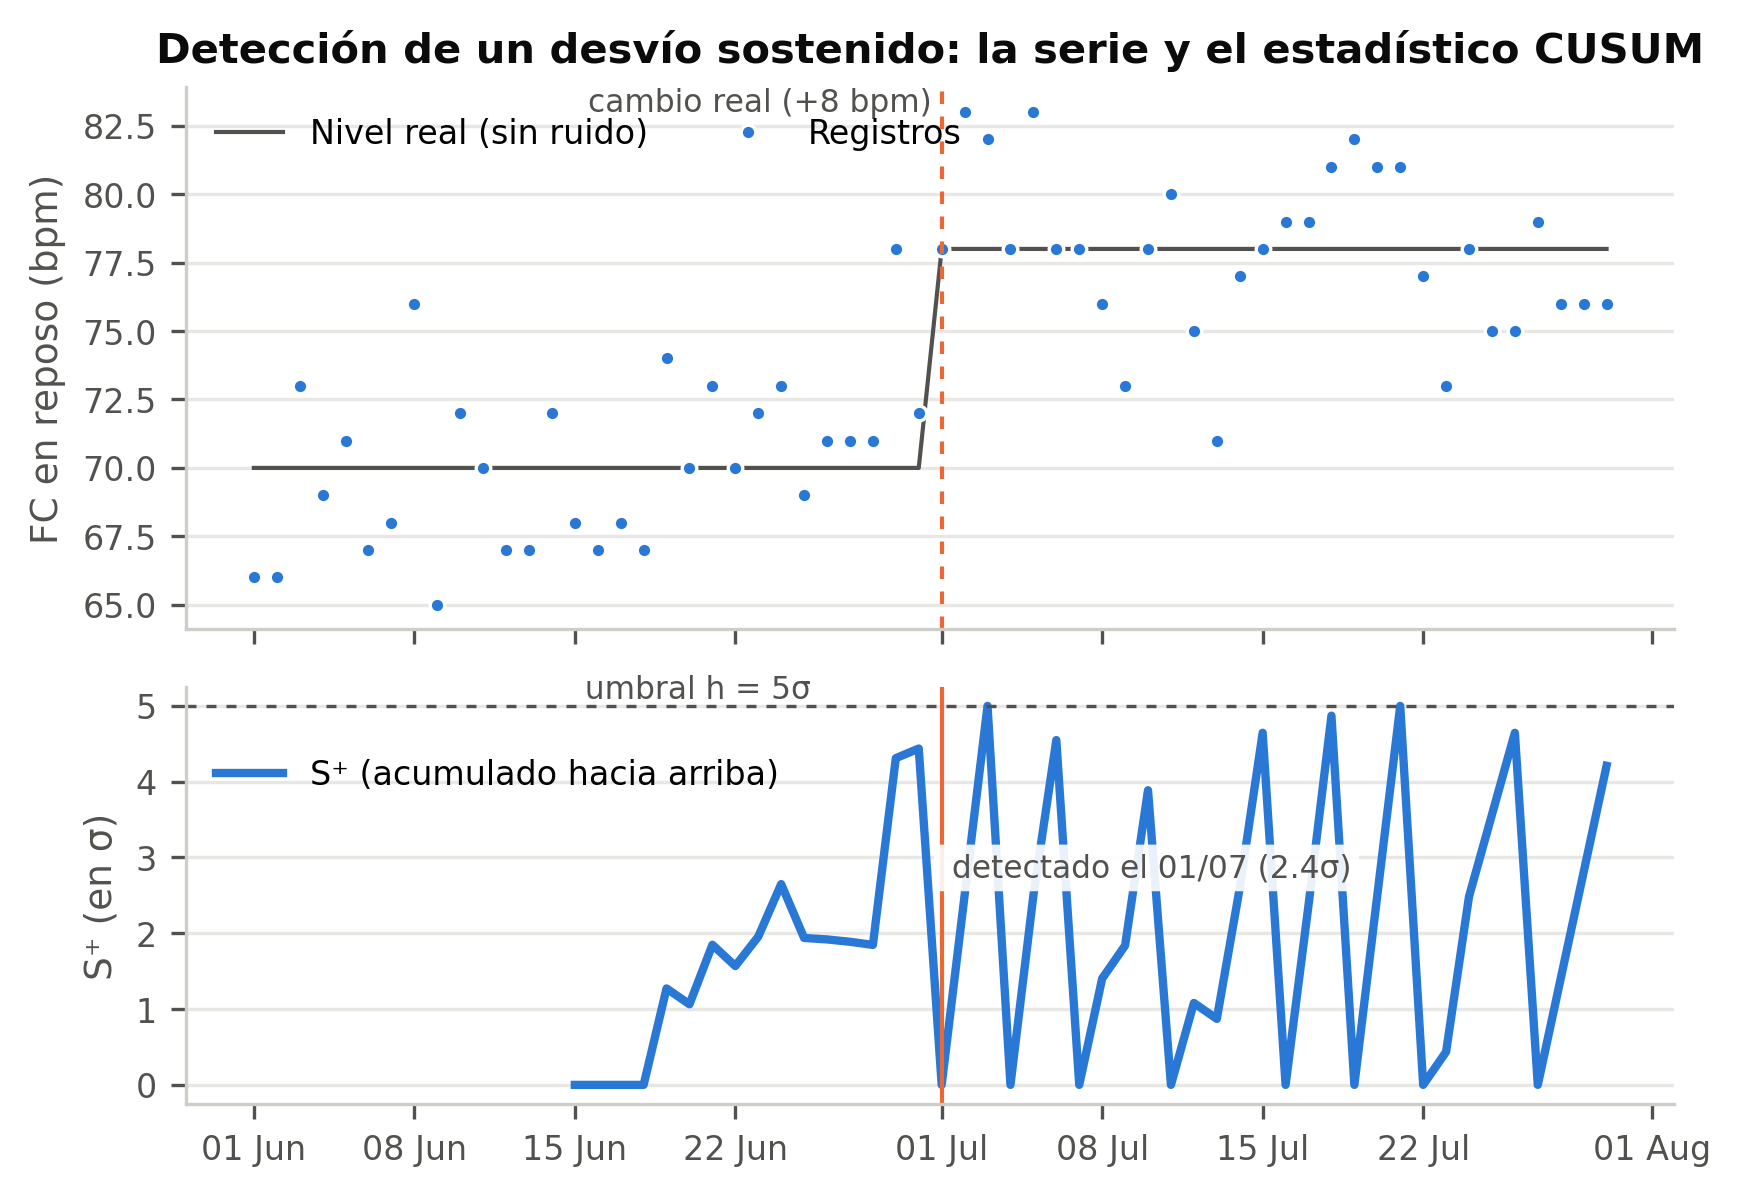
\includegraphics[width=0.84\linewidth]{fig3-cusum-deteccion.png}
\notaAPA{Serie sintética de 60 días con un salto de +8 lpm el día 30. Arriba, los
registros y el nivel real; abajo, el estadístico acumulado $S^{+}$ y el umbral
$h=5$.}
\end{figure}

\subsection{Estimador de Riesgo sobre NHANES}
\label{sec:nhanes-resultados}

La Tabla~\ref{tab:auc} y la Figura~\ref{fig:auc} presentan el desempeño de los
once modelos sobre las mismas 50 particiones de prueba, y la
Tabla~\ref{tab:delta} contrasta los pares que responden a las preguntas P3 y P4.

\begin{table}[!htbp]
\tablaAPA{tab:auc}{Discriminación del antecedente cardiovascular en NHANES 2021-2023}
\small
\noindent\begin{tabularx}{\linewidth}{P{4.3cm}Lcc}
\hline
\textbf{Modelo} & \textbf{Variables} & \textbf{AUC} & \textbf{Brier} \\
\hline
\multicolumn{4}{l}{\textit{Benchmarks}} \\
Prevalencia & ninguna & 0,500 $\pm$ 0,000 & 0,104 \\
Regresión logística & edad y sexo & 0,769 $\pm$ 0,013 & 0,094 \\
\multicolumn{4}{l}{\textit{Sin entrenamiento}} \\
Heurística inicial & FC, sueño, estrés & 0,564 $\pm$ 0,026 & -- \\
Índice del motor & FC, sueño, estrés, IMC, tabaco & 0,611 $\pm$ 0,025 & -- \\
Índice del motor + contexto & índice, edad y sexo & 0,799 $\pm$ 0,015 & -- \\
\multicolumn{4}{l}{\textit{Entrenados sobre NHANES}} \\
Regresión logística & estilo de vida (5) & 0,608 $\pm$ 0,025 & 0,103 \\
Gradient boosting & estilo de vida (5) & 0,605 $\pm$ 0,025 & 0,105 \\
Regresión logística & estilo de vida, edad y sexo (7) & \textbf{0,805 $\pm$ 0,014} & \textbf{0,091} \\
Regresión logística & los 7 log RR del motor & 0,801 $\pm$ 0,015 & 0,092 \\
Gradient boosting & estilo de vida, edad y sexo (7) & 0,794 $\pm$ 0,016 & 0,093 \\
k vecinos ($k=65$) & estilo de vida, edad y sexo (7) & 0,775 $\pm$ 0,017 & 0,094 \\
\hline
\end{tabularx}
\notaAPA{AUC: área bajo la curva ROC, media $\pm$ desvío sobre 50 particiones de
prueba (validación cruzada estratificada 5\,$\times$\,10, $n=5.043$). Brier: error
cuadrático medio de la probabilidad, solo para los modelos que la producen. El
estilo de vida comprende frecuencia cardíaca, IMC, sueño, PHQ-9 y tabaquismo. El
índice sin entrenamiento se evalúa por su orden: a mayor riesgo relativo, mayor
riesgo.}
\end{table}

\begin{figure}[!htbp]
\figuraAPA{fig:auc}{Área bajo la curva ROC de todos los modelos sobre NHANES}
\centering
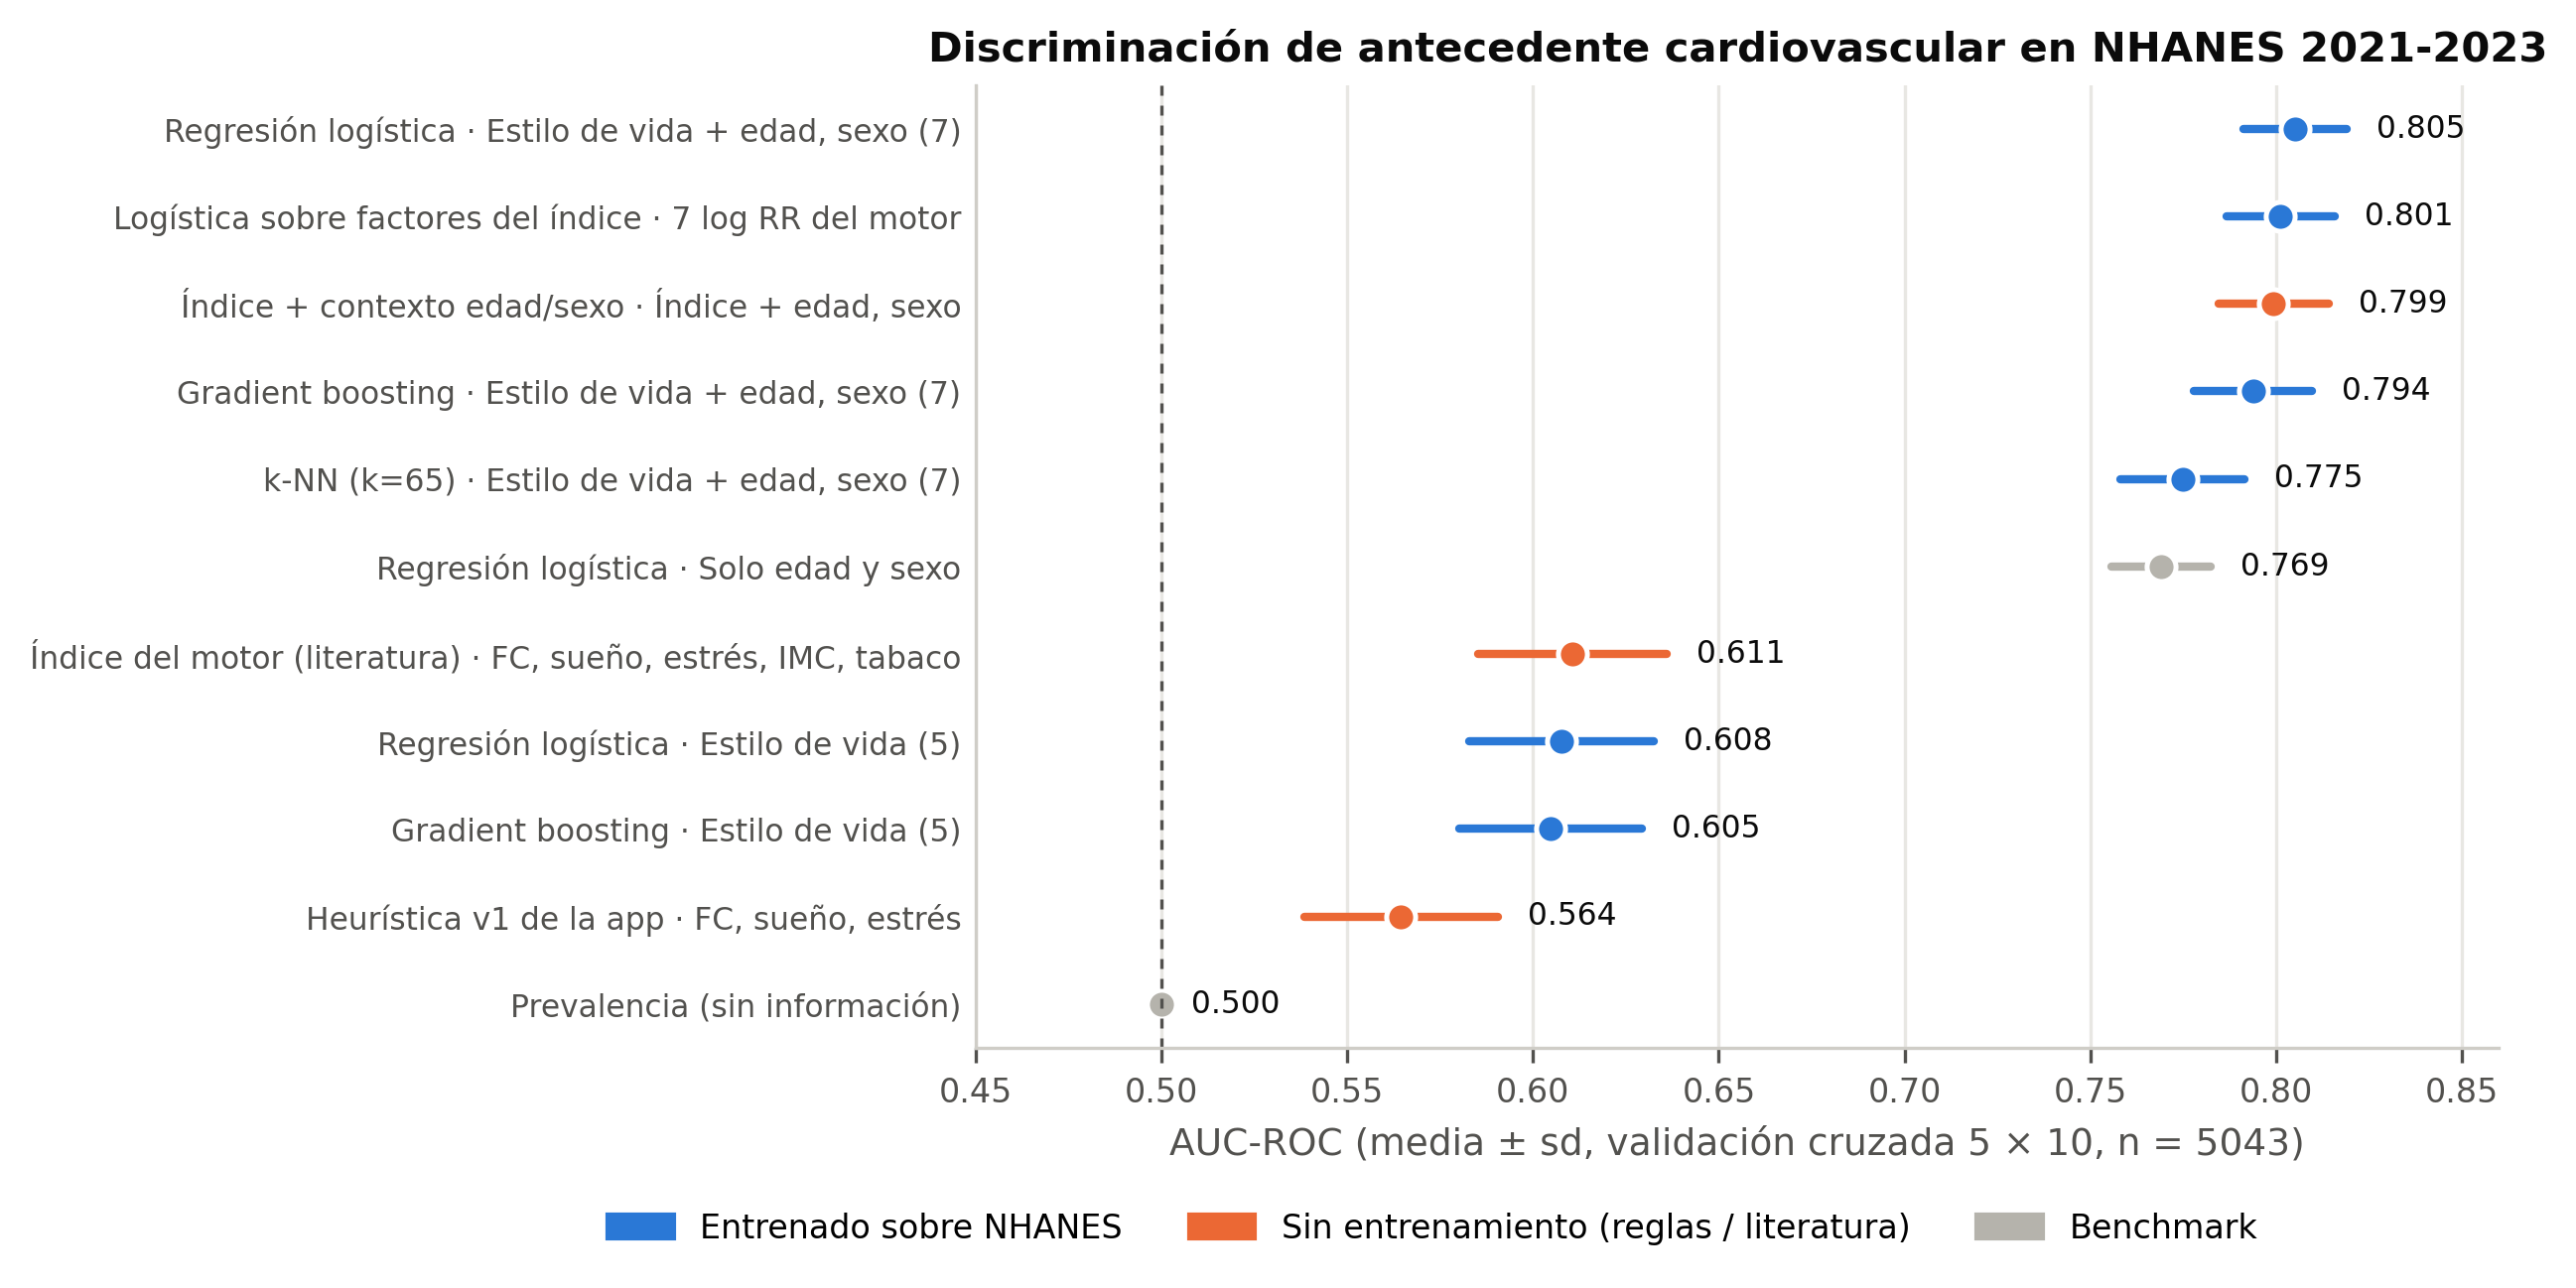
\includegraphics[width=0.95\linewidth]{fig8-auc-nhanes.png}
\notaAPA{Media $\pm$ desvío sobre 50 particiones de prueba. En azul los modelos
entrenados, en naranja los puntajes sin entrenamiento y en gris los benchmarks.}
\end{figure}

\begin{table}[!htbp]
\tablaAPA{tab:delta}{Diferencias de área bajo la curva entre pares de modelos}
\small
\noindent\begin{tabularx}{\linewidth}{Lcc}
\hline
\textbf{Comparación} & \textbf{$\Delta$AUC} & \textbf{IC 95\,\%} \\
\hline
Índice del motor frente a la heurística inicial & +0,046 & [0,016; 0,075] \\
Logística con estilo de vida frente al índice del motor & $-0{,}001$ & [$-0{,}022$; 0,019] \\
Logística con estilo de vida, edad y sexo frente a solo edad y sexo & +0,037 & [0,025; 0,049] \\
Logística con estilo de vida, edad y sexo frente al índice + contexto & +0,007 & [$-0{,}001$; 0,015] \\
Gradient boosting frente a logística, ambos con 7 variables & $-0{,}010$ & [$-0{,}018$; $-0{,}001$] \\
\hline
\end{tabularx}
\notaAPA{Diferencia sobre las predicciones fuera de muestra de la primera
repetición; intervalo por bootstrap pareado de 2.000 remuestreos. Un intervalo
que no contiene el cero indica una diferencia significativa al 5\,\%.}
\end{table}

\textbf{Los indicadores de estilo de vida discriminan poco por sí solos.} Con
las cinco variables modificables, el mejor modelo alcanza un AUC de 0,61. La
frecuencia cardíaca en reposo, por ejemplo, tiene la misma media en quienes
tienen antecedente y en quienes no lo tienen (70,8 y 70,7 lpm,
Tabla~\ref{tab:descriptiva}). Aun así, el índice del motor ordena mejor que la
heurística inicial ($\Delta$AUC $=+0{,}046$, intervalo que excluye el cero), lo
que confirma empíricamente el reemplazo de los umbrales fijos por funciones
continuas y la incorporación del IMC y del tabaquismo.

\textbf{Entrenar no mejora al índice de la literatura (P4).} Una regresión
logística entrenada con las mismas variables obtiene 0,608 frente a 0,611 del
índice, una diferencia de $-0{,}001$ con un intervalo centrado en cero. Con edad y
sexo, el índice combinado con su contexto alcanza 0,799 y la regresión logística
entrenada 0,805: la ventaja de 0,007 no es significativa al 5\,\%. El índice,
construido solo con coeficientes publicados y sin ver estos datos, ordena a las
personas prácticamente igual que el mejor modelo entrenado.

\textbf{Edad y sexo son el factor decisivo, pero no el único (P3).} La regresión
logística con solo edad y sexo ya alcanza 0,769; agregar las cinco variables de
estilo de vida la lleva a 0,805, una mejora de 0,037 con un intervalo de
[0,025; 0,049]. Las variables que la aplicación captura sí aportan información
por encima de la demografía. Esto motivó la incorporación del perfil opcional
con edad y sexo.

\textbf{La relación es esencialmente lineal.} El gradient boosting no supera a la
regresión logística; con siete variables queda 0,010 por debajo, diferencia
significativa, y k vecinos queda en 0,775. No hay evidencia de interacciones o no
linealidades que justifiquen un modelo más flexible, y la regresión logística
tiene la ventaja de producir coeficientes interpretables.

\begin{figure}[!htbp]
\figuraAPA{fig:roc}{Curvas ROC sobre NHANES 2021-2023}
\centering
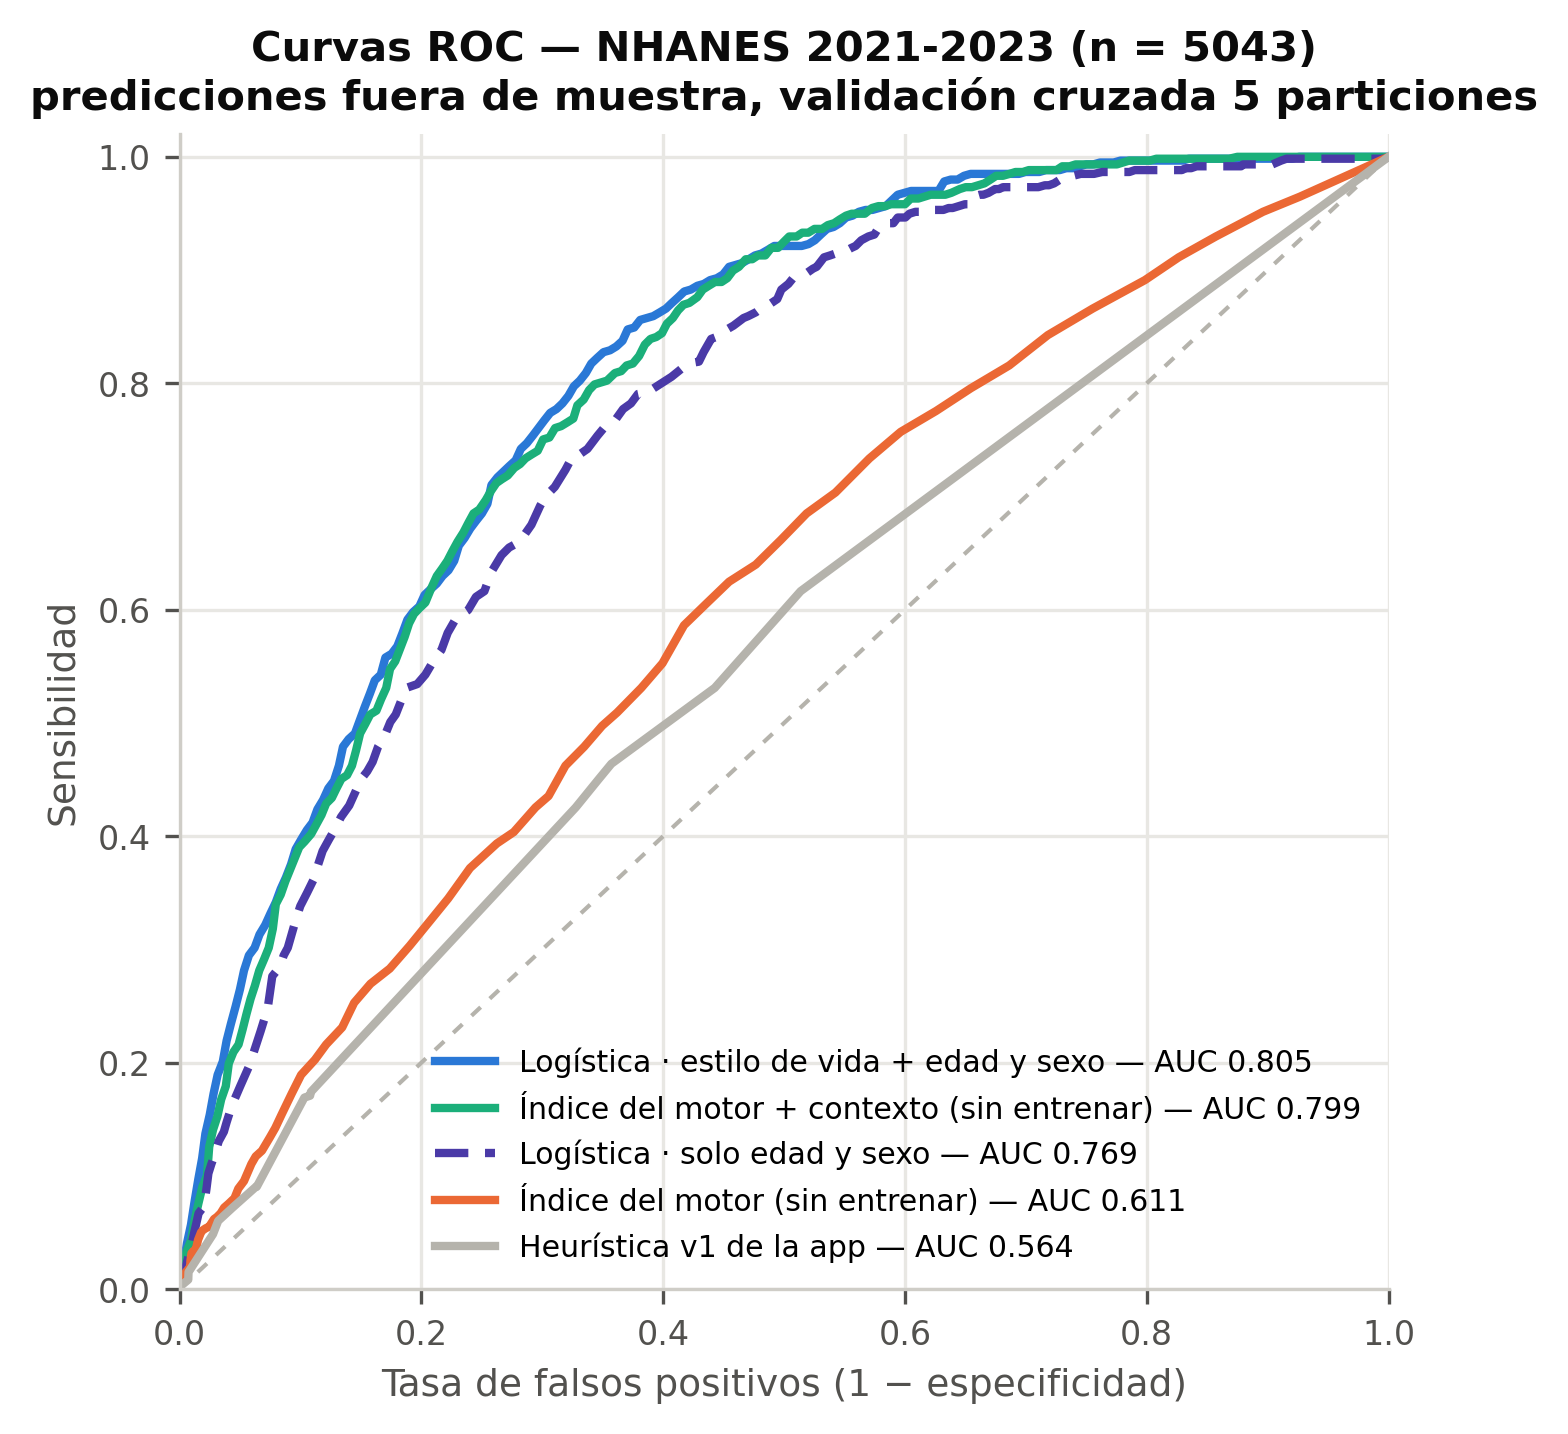
\includegraphics[width=0.6\linewidth]{fig9-roc-nhanes.png}
\notaAPA{Predicciones fuera de muestra de la primera repetición de la validación
cruzada. Las curvas del índice con contexto y de la regresión logística
entrenada prácticamente se superponen.}
\end{figure}

\textbf{Calibración y punto de operación.} Las probabilidades de la regresión
logística de referencia, con estilo de vida, edad y sexo, están bien calibradas
(Figura~\ref{fig:calibracion}): la pendiente de calibración es 0,99 y el
intercepto $-0{,}02$, frente a los valores ideales de 1 y 0, y el riesgo medio
predicho coincide con la prevalencia observada, 11,8\,\%. El puntaje de Brier
baja de 0,104 con la prevalencia a 0,091, una mejora del 13\,\%. En el umbral de
Youden, una probabilidad de 0,11, la sensibilidad es 0,822 y la especificidad
0,656, con un valor predictivo negativo de 0,965 y uno positivo de 0,243. Por
eso la herramienta sirve para descartar más que para confirmar. El umbral se
eligió sobre las mismas predicciones que se evalúan, por lo que esas dos cifras
son levemente optimistas.

\begin{figure}[!htbp]
\figuraAPA{fig:calibracion}{Calibración por deciles de riesgo predicho}
\centering
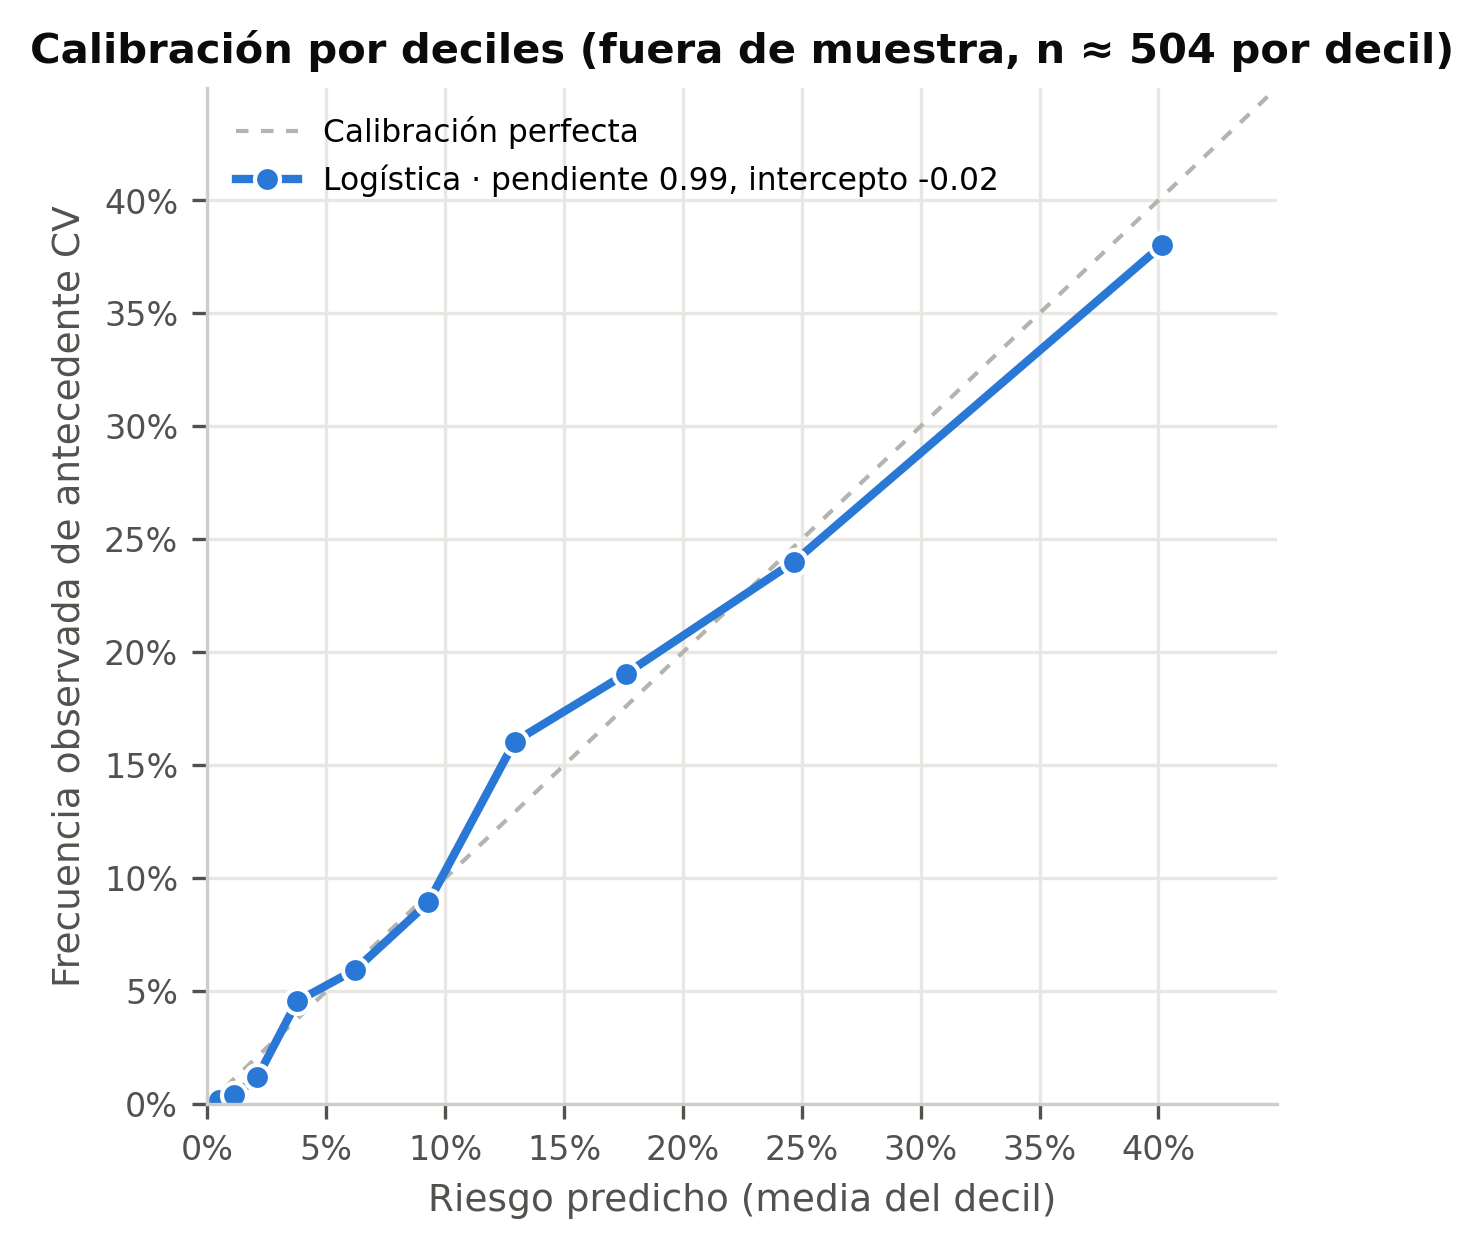
\includegraphics[width=0.52\linewidth]{fig10-calibracion-nhanes.png}
\notaAPA{Regresión logística con estilo de vida, edad y sexo; predicciones fuera
de muestra agrupadas en diez deciles de alrededor de 504 personas.}
\end{figure}

\textbf{Coeficientes.} La Tabla~\ref{tab:or} presenta los odds ratio del modelo
de referencia ajustado a los 5.043 adultos, en ocho iteraciones de IRLS. Todos
los coeficientes son significativos y, salvo el del sueño, que se discute en la
nota, tienen el signo esperado. La edad domina, con un odds ratio de 4,06 por
desvío estándar, seguida del IMC (1,46) y del PHQ-9 (1,39). El odds ratio por
década, 2,27 [2,09; 2,47], es cercano a la regla de duplicación por década que
usa el contexto del índice, aunque algo mayor: el intervalo no incluye el 2.

\begin{table}[!htbp]
\tablaAPA{tab:or}{Odds ratio de la regresión logística con estilo de vida, edad y sexo}
\small
\noindent\begin{tabularx}{\linewidth}{Lccccc}
\hline
\textbf{Variable} & \textbf{OR por 1 DE} & \textbf{IC 95\,\%} & \textbf{OR} & \textbf{IC 95\,\%} & \textbf{Unidad} \\
\hline
Edad & 4,06 & 3,51--4,69 & 2,27 & 2,09--2,47 & +10 años \\
IMC & 1,46 & 1,33--1,60 & 1,30 & 1,22--1,39 & +5 kg/m\textsuperscript{2} \\
Sexo masculino & 1,41 & 1,28--1,55 & 2,00 & 1,65--2,41 & hombre/mujer \\
PHQ-9 & 1,39 & 1,27--1,52 & 1,43 & 1,30--1,57 & +5 puntos \\
Fumador actual & 1,24 & 1,14--1,35 & 1,85 & 1,44--2,37 & sí/no \\
Sueño & 1,14 & 1,04--1,24 & 1,09 & 1,03--1,15 & +1 h \\
FC en reposo & 1,11 & 1,01--1,21 & 1,08 & 1,01--1,17 & +10 lpm \\
\hline
\end{tabularx}
\notaAPA{DE: desvío estándar de la variable en la muestra. Todos los coeficientes
tienen $p<0{,}05$; el de la frecuencia cardíaca es el menos significativo
($p=0{,}035$). El odds ratio del sueño es positivo porque el sueño largo también
se asocia con mayor riesgo y porque, en un diseño transversal, está confundido
por la edad y la morbilidad previa.}
\end{table}

\textbf{Recalibración del índice.} Para saber si los coeficientes de la
literatura están bien dimensionados, se entrenó una regresión logística cuyas
variables son los siete componentes del índice, es decir, los cinco log-riesgos
relativos de los factores y los dos del contexto. Si la literatura acertara la
magnitud de un factor, su peso aprendido valdría 1. La Figura~\ref{fig:pesos}
muestra que los pesos de la frecuencia cardíaca, el sueño y el IMC son
compatibles con 1, porque sus intervalos lo contienen; el sueño da exactamente
1,00. El estrés aproximado por PHQ-9 (5,32), la edad (1,28) y el sexo (1,58)
pesan más de lo que asigna el índice, y el tabaquismo menos (0,70). Dos de esas
diferencias son compatibles con el diseño transversal: quien ya tuvo un evento
suele dejar de fumar y presenta más síntomas depresivos, lo que debilita el
primer coeficiente y refuerza el segundo sin que eso diga algo sobre el riesgo
futuro. En conjunto, reajustar los siete pesos lleva el AUC de 0,799 a 0,801: el
orden que produce el índice ya es prácticamente el óptimo para estas variables,
y no hay evidencia suficiente para reemplazar los coeficientes publicados por
coeficientes estimados en un estudio transversal.

\begin{figure}[!htbp]
\figuraAPA{fig:pesos}{Pesos aprendidos para cada componente del índice}
\centering
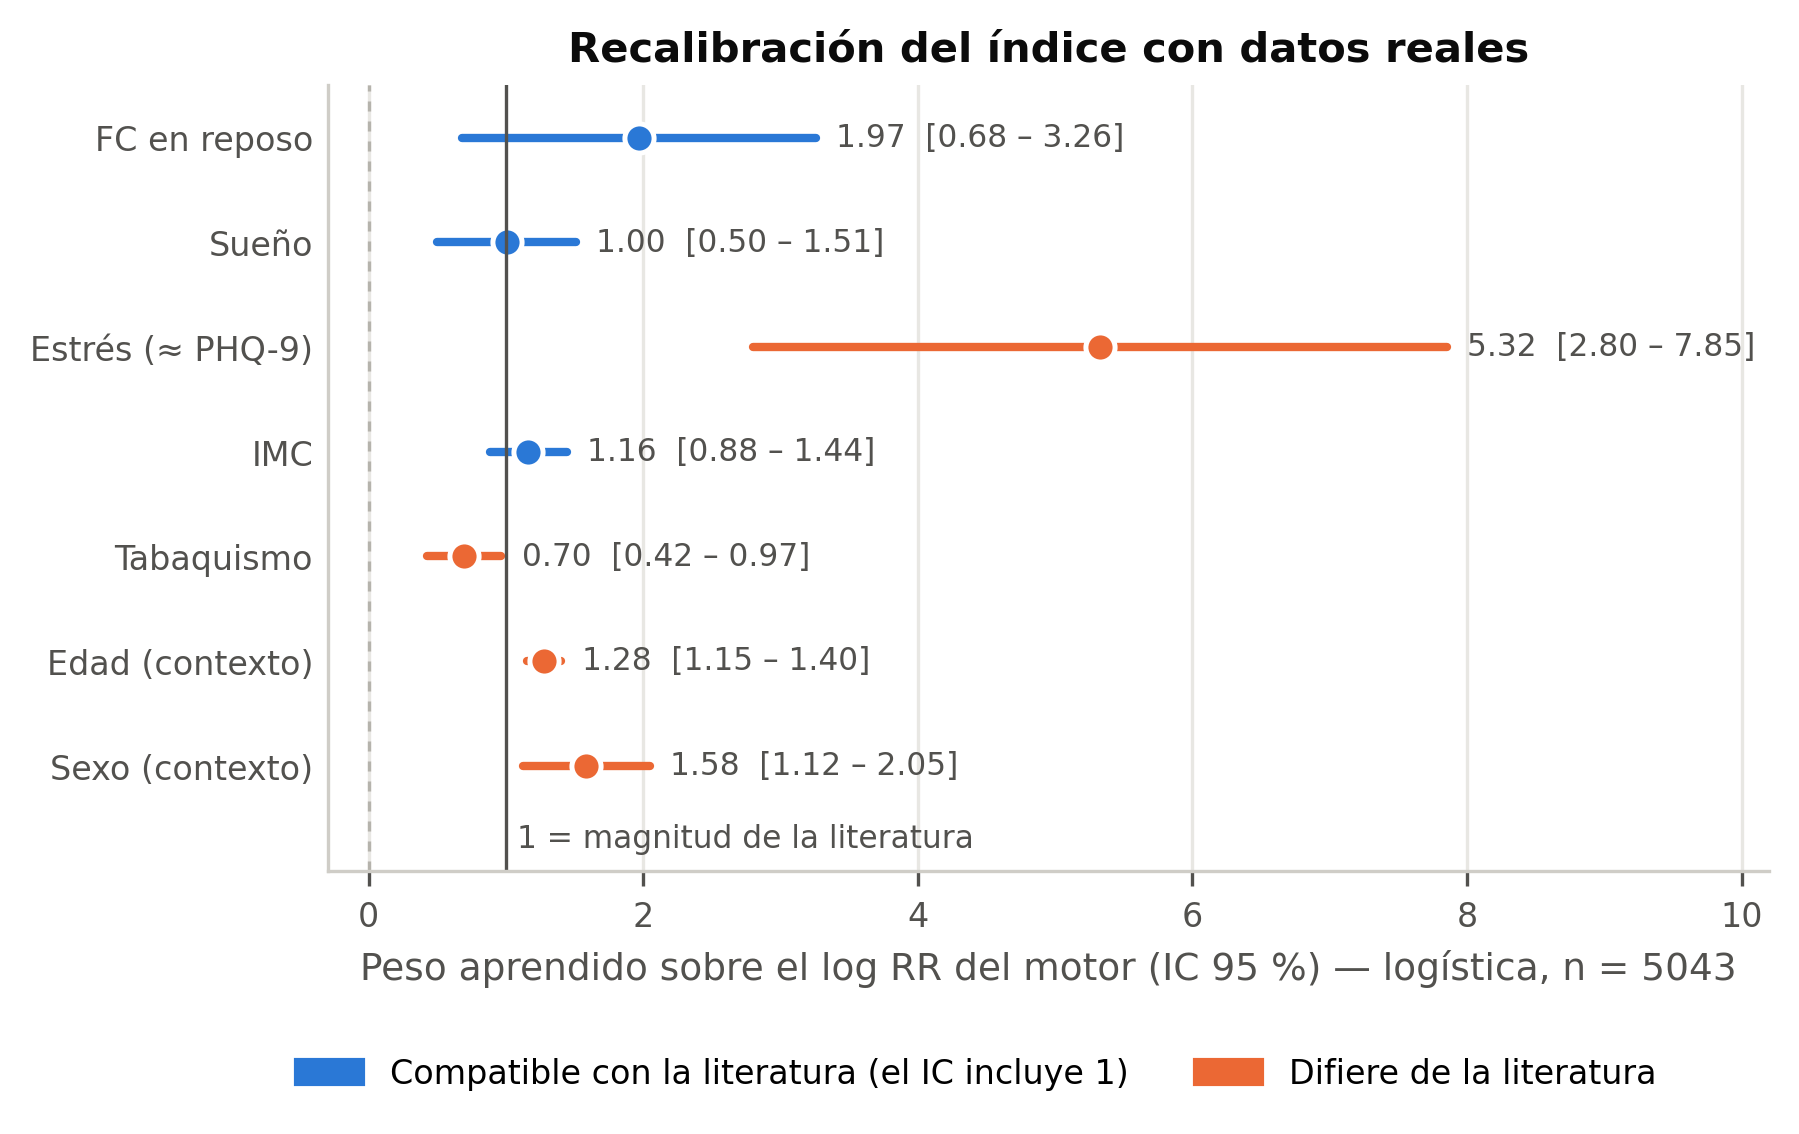
\includegraphics[width=0.84\linewidth]{fig11-pesos-indice-nhanes.png}
\notaAPA{Peso de cada log-riesgo relativo del motor en una regresión logística
ajustada a los 5.043 adultos, con su intervalo de confianza del 95\,\%. Un peso de
1 significa que la magnitud de la literatura coincide con la de los datos.}
\end{figure}

\textbf{Trazabilidad del avance anterior.} La versión previa de este documento
reportaba, para una partición única de prueba del 30\,\%, un AUC de 0,605 con las
variables de la aplicación y de 0,812 al agregar edad y sexo. Esa especificación
se replicó con el código del proyecto sobre la misma muestra, que coincide
exactamente (5.043 adultos y 597 casos). Las medias de validación cruzada,
0,603 y 0,803, son prácticamente iguales a las reportadas, 0,600 y 0,802. En la
partición única se obtuvieron 0,615 y 0,795; la diferencia con lo reportado es
compatible con la variabilidad de una sola partición, cuyo desvío entre
particiones es del orden de 0,025 y 0,014 (Tabla~\ref{tab:auc}). La heurística
inicial da 0,5645 sobre la muestra completa, el mismo valor reportado (0,565). Por
esa variabilidad, este documento reporta la validación cruzada repetida en lugar
de una partición única.

\subsection{Validación de la Implementación sobre UCI}
\label{sec:uci-resultados}

Sobre el conjunto de Cleveland, la regresión logística con las 13 variables
clínicas alcanza un AUC de 0,904 (Tabla~\ref{tab:uci}) y supera a k vecinos
(0,880). Con solo edad, sexo y frecuencia cardíaca máxima baja a 0,785, lo que
cuantifica cuánto aportan el electrocardiograma y la prueba de esfuerzo. La
reimplementación independiente en numpy reproduce los coeficientes y errores
estándar de la implementación propia con una diferencia máxima de
$2\times 10^{-14}$ en UCI y de $6\times 10^{-15}$ en NHANES, del orden del error
de redondeo de la aritmética de doble precisión. En esta cohorte la edad no
resulta significativa ($p=0{,}38$) y el sexo masculino tiene un odds ratio de 6,0.
Son rasgos de una cohorte de derivación cardiológica, no de la población
general, y justifican que el estimador de la aplicación no se construya sobre
estos datos.

\begin{table}[!htbp]
\tablaAPA{tab:uci}{Validación cruzada sobre UCI Heart Disease (Cleveland)}
\small
\noindent\begin{tabularx}{\linewidth}{P{3.8cm}Lcc}
\hline
\textbf{Modelo} & \textbf{Variables} & \textbf{AUC} & \textbf{Brier} \\
\hline
Prevalencia & ninguna & 0,500 $\pm$ 0,000 & 0,249 \\
Regresión logística & edad, sexo, FC máxima (3) & 0,785 $\pm$ 0,058 & 0,190 \\
Regresión logística & clínico básico (6) & 0,795 $\pm$ 0,056 & 0,185 \\
Regresión logística & completo (13) & \textbf{0,904 $\pm$ 0,032} & \textbf{0,124} \\
k vecinos ($k=7$) & completo (13) & 0,880 $\pm$ 0,042 & 0,139 \\
\hline
\end{tabularx}
\notaAPA{$n=297$; validación cruzada estratificada 5\,$\times$\,10. El conjunto
clínico básico agrega presión sistólica, colesterol y glucemia en ayunas.}
\end{table}

\subsection{Consecuencias para el Diseño}

Los resultados se tradujeron en decisiones concretas sobre la aplicación:

\begin{itemize}
  \item El puntaje heurístico inicial se reemplazó por el índice del motor, que
    discrimina mejor con diferencia significativa.
  \item Se mantienen los coeficientes de la literatura: entrenarlos sobre NHANES
    no mejora el orden y los introduciría con los sesgos de un diseño
    transversal.
  \item La aplicación incorpora un perfil opcional con edad, sexo, altura y
    tabaquismo, porque la edad y el sexo son los predictores más fuertes y el IMC
    y el tabaquismo aportan sobre ellos.
  \item La edad y el sexo se muestran como contexto y no dentro del puntaje: la
    combinación de ambos conserva la discriminación (0,799) sin que el puntaje
    castigue lo que la persona no puede modificar.
  \item El pronóstico se selecciona por serie y por usuario, porque ningún
    modelo gana en todas: en 8 de las 28 series el mejor fue un benchmark.
\end{itemize}

\newpage

%======================= 9. CONCLUSIONES =======================
\section{Conclusiones}
\label{sec:conclusiones}

Las enfermedades cardiovasculares constituyen, simultáneamente, un desafío
médico, tecnológico y social. La detección tardía del riesgo, las barreras de
acceso a servicios preventivos y la baja alfabetización en salud configuran un
escenario que demanda soluciones integrales. Desde la ingeniería de sistemas,
este trabajo muestra que el aporte técnico de una plataforma preventiva no está
en conectar un modelo de lenguaje, sino en construir y evaluar el sistema que
produce las cifras.

El motor de predicción de Pulso resuelve ese problema con componentes
implementados desde cero y medidos contra benchmarks. En pronóstico, el modelo
seleccionado supera al pronóstico ingenuo en 23 de 28 series y recupera las
pendientes y patrones semanales verdaderos. En detección, CUSUM identifica los
cuatro cambios de régimen con 4,5 días de retraso medio. En estimación de riesgo,
sobre 5.043 adultos reales, el índice construido con coeficientes publicados
supera a la heurística inicial y rinde igual que una regresión logística
entrenada con las mismas variables; con edad y sexo alcanza un AUC de 0,799,
frente a 0,805 del mejor modelo entrenado, que además está calibrado.

El trabajo también responde con cifras una pregunta que la literatura de
prototipos de salud digital suele dejar implícita: cuánto riesgo cardiovascular
puede estimarse sin laboratorio. Los indicadores de estilo de vida, solos,
discriminan de forma limitada (0,61); la edad y el sexo explican la mayor parte
de la discriminación alcanzable (0,77); y las variables que la aplicación
registra agregan una mejora pequeña pero significativa sobre ellas (+0,037).
Reconocer y cuantificar esa restricción, en lugar de sortearla, delimita con
honestidad el alcance del prototipo y orientó su rediseño.

Como trabajo de grado, el proyecto aporta a la salud digital y a la ingeniería de
sistemas aplicada al sector salud, y se alinea con los Objetivos de Desarrollo
Sostenible vinculados a salud y bienestar, reducción de desigualdades e
innovación. Las siguientes fases abordarán la validación del pronóstico con
series reales de dispositivos portátiles, la validación externa y la
recalibración del estimador en población colombiana, un diseño longitudinal que
permita predicción prospectiva, la incorporación de los ponderadores muestrales
de NHANES y la validación con usuarios representativos y con la revisión de un
profesional de la salud.

\newpage

%======================= REFERENCIAS =======================
\section*{REFERENCIAS}
\addcontentsline{toc}{section}{Referencias}

\begin{enumerate}[label={[\arabic*]}, leftmargin=2.2em]

\item Abramowitz, M., \& Stegun, I. A. (Eds.). (1964). \textit{Handbook of
mathematical functions with formulas, graphs, and mathematical tables}. National
Bureau of Standards.

\item Aune, D., Sen, A., ó'Hartaigh, B., Janszky, I., Romundstad, P. R.,
Tonstad, S., \& Vatten, L. J. (2017). Resting heart rate and the risk of
cardiovascular disease, total cancer, and all-cause mortality: A systematic
review and dose-response meta-analysis of prospective studies.
\textit{Nutrition, Metabolism and Cardiovascular Diseases, 27}(6), 504--517.
\url{https://doi.org/10.1016/j.numecd.2017.04.004}

\item Biduski, D., Bellei, E. A., Rodriguez, J. P. M., Zaina, L. A. M., \& De
Marchi, A. C. B. (2020). Assessing long-term user experience on a mobile health
application through an in-app embedded conversation-based questionnaire.
\textit{Computers in Human Behavior, 104}, 106169.
\url{https://doi.org/10.1016/j.chb.2019.106169}

\item Cappuccio, F. P., Cooper, D., D'Elia, L., Strazzullo, P., \& Miller, M. A.
(2011). Sleep duration predicts cardiovascular outcomes: A systematic review and
meta-analysis of prospective studies. \textit{European Heart Journal, 32}(12),
1484--1492. \url{https://doi.org/10.1093/eurheartj/ehr007}

\item Centers for Disease Control and Prevention, National Center for Health
Statistics. (2024). \textit{National Health and Nutrition Examination Survey:
August 2021 -- August 2023 data files} [Conjunto de datos]. U.S. Department of
Health and Human Services.
\url{https://wwwn.cdc.gov/nchs/nhanes/continuousnhanes/default.aspx?Cycle=2021-2023}

\item Cover, T., \& Hart, P. (1967). Nearest neighbor pattern classification.
\textit{IEEE Transactions on Information Theory, 13}(1), 21--27.
\url{https://doi.org/10.1109/TIT.1967.1053964}

\item Dawber, T. R., Meadors, G. F., \& Moore, F. E. (1951). Epidemiological
approaches to heart disease: The Framingham Study. \textit{American Journal of
Public Health, 41}(3), 279--281. \url{https://doi.org/10.2105/AJPH.41.3.279}

\item Detrano, R., Janosi, A., Steinbrunn, W., Pfisterer, M., Schmid, J.,
Sandhu, S., Guppy, K., Lee, S., \& Froelicher, V. (1989). International
application of a new probability algorithm for the diagnosis of coronary artery
disease. \textit{American Journal of Cardiology, 64}(5), 304--310.
\url{https://doi.org/10.1016/0002-9149(89)90524-9}

\item Efron, B., \& Tibshirani, R. J. (1993). \textit{An introduction to the
bootstrap}. Chapman \& Hall.

\item Friedman, J. H. (2001). Greedy function approximation: A gradient boosting
machine. \textit{The Annals of Statistics, 29}(5), 1189--1232.
\url{https://doi.org/10.1214/aos/1013203451}

\item Gardner, E. S., Jr., \& McKenzie, E. (1985). Forecasting trends in time
series. \textit{Management Science, 31}(10), 1237--1246.
\url{https://doi.org/10.1287/mnsc.31.10.1237}

\item Global BMI Mortality Collaboration. (2016). Body-mass index and all-cause
mortality: Individual-participant-data meta-analysis of 239 prospective studies
in four continents. \textit{The Lancet, 388}(10046), 776--786.
\url{https://doi.org/10.1016/S0140-6736(16)30175-1}

\item Hanley, J. A., \& McNeil, B. J. (1982). The meaning and use of the area
under a receiver operating characteristic (ROC) curve. \textit{Radiology,
143}(1), 29--36. \url{https://doi.org/10.1148/radiology.143.1.7063747}

\item Hastie, T., Tibshirani, R., \& Friedman, J. (2009). \textit{The elements
of statistical learning: Data mining, inference, and prediction} (2.\textsuperscript{a} ed.).
Springer. \url{https://doi.org/10.1007/978-0-387-84858-7}

\item Hawkins, D. M. (1987). Self-starting CUSUM charts for location and scale.
\textit{Journal of the Royal Statistical Society: Series D (The Statistician),
36}(4), 299--316.

\item Hawkins, D. M., \& Olwell, D. H. (1998). \textit{Cumulative sum charts and
charting for quality improvement}. Springer.
\url{https://doi.org/10.1007/978-1-4612-1686-5}

\item Holt, C. C. (2004). Forecasting seasonals and trends by exponentially
weighted moving averages. \textit{International Journal of Forecasting, 20}(1),
5--10. \url{https://doi.org/10.1016/j.ijforecast.2003.09.015} (Trabajo original
publicado en 1957)

\item Hyndman, R. J., \& Athanasopoulos, G. (2021). \textit{Forecasting:
Principles and practice} (3.\textsuperscript{a} ed.). OTexts. \url{https://otexts.com/fpp3/}

\item Hyndman, R. J., \& Koehler, A. B. (2006). Another look at measures of
forecast accuracy. \textit{International Journal of Forecasting, 22}(4),
679--688. \url{https://doi.org/10.1016/j.ijforecast.2006.03.001}

\item Janosi, A., Steinbrunn, W., Pfisterer, M., \& Detrano, R. (1988).
\textit{Heart Disease} [Conjunto de datos]. UCI Machine Learning Repository.
\url{https://doi.org/10.24432/C52P4X}

\item Krittanawong, C., Virk, H. U. H., Bangalore, S., Wang, Z., Johnson, K. W.,
Pinotti, R., Zhang, H., Kaplin, S., Narasimhan, B., Kitai, T., Baber, U.,
Halperin, J. L., \& Tang, W. H. W. (2020). Machine learning prediction in
cardiovascular diseases: A meta-analysis. \textit{Scientific Reports, 10}(1),
16057. \url{https://doi.org/10.1038/s41598-020-72685-1}

\item Kroenke, K., Spitzer, R. L., \& Williams, J. B. W. (2001). The PHQ-9:
Validity of a brief depression severity measure. \textit{Journal of General
Internal Medicine, 16}(9), 606--613.
\url{https://doi.org/10.1046/j.1525-1497.2001.016009606.x}

\item le Cessie, S., \& van Houwelingen, J. C. (1992). Ridge estimators in
logistic regression. \textit{Journal of the Royal Statistical Society: Series C
(Applied Statistics), 41}(1), 191--201. \url{https://doi.org/10.2307/2347628}

\item Liao, P., Greenewald, K., Klasnja, P., \& Murphy, S. (2020). Personalized
HeartSteps: A reinforcement learning algorithm for optimizing physical activity.
\textit{Proceedings of the ACM on Interactive, Mobile, Wearable and Ubiquitous
Technologies, 4}(1), 1--22. \url{https://doi.org/10.1145/3381007}

\item Ministerio de Salud y Protección Social de Colombia. (2022).
\textit{Análisis de Situación de Salud (ASIS) Colombia}. Bogotá D.C.
\url{https://www.minsalud.gov.co}

\item Montgomery, D. C. (2019). \textit{Introduction to statistical quality
control} (8.\textsuperscript{a} ed.). Wiley.

\item National Heart, Lung, and Blood Institute. (2026). \textit{Framingham
Heart Study: Three generations of dedication} [Sitio web]. Recuperado el 15 de
agosto de 2026, de \url{https://www.framinghamheartstudy.org}

\item Observatorio Nacional de Salud. (2021). \textit{Informe sobre enfermedades
cardiovasculares en Colombia}. Instituto Nacional de Salud.
\url{https://www.ins.gov.co}

\item Organización Mundial de la Salud. (2026a). \textit{Cardiovascular diseases
(CVDs): Key facts}. OMS.
\url{https://www.who.int/news-room/fact-sheets/detail/cardiovascular-diseases-cvds}

\item Organización Mundial de la Salud. (2026b). \textit{Global Health
Observatory} [Repositorio de datos]. Recuperado el 15 de agosto de 2026, de
\url{https://www.who.int/data/gho}

\item Page, E. S. (1954). Continuous inspection schemes. \textit{Biometrika,
41}(1--2), 100--115. \url{https://doi.org/10.1093/biomet/41.1-2.100}

\item Pinzón, A., Aristizábal, J. C., Cubillos-Garzón, L. A., González, C., \&
Lara-Díaz, M. F. (2020). Factores de riesgo cardiovascular en población adulta
colombiana: brechas en tamizaje y prevención. \textit{Revista Colombiana de
Cardiología, 27}(4), 263--272.

\item Richardson, S., Shaffer, J. A., Falzon, L., Krupka, D., Davidson, K. W.,
\& Edmondson, D. (2012). Meta-analysis of perceived stress and its association
with incident coronary heart disease. \textit{American Journal of Cardiology,
110}(12), 1711--1716. \url{https://doi.org/10.1016/j.amjcard.2012.08.004}

\item Roberts, S. W. (1959). Control chart tests based on geometric moving
averages. \textit{Technometrics, 1}(3), 239--250.
\url{https://doi.org/10.1080/00401706.1959.10489860}

\item Sen, P. K. (1968). Estimates of the regression coefficient based on
Kendall's tau. \textit{Journal of the American Statistical Association,
63}(324), 1379--1389. \url{https://doi.org/10.1080/01621459.1968.10480934}

\item Theil, H. (1950). A rank-invariant method of linear and polynomial
regression analysis, I. \textit{Proceedings of the Royal Netherlands Academy of
Sciences, 53}, 386--392.

\item Van Calster, B., McLernon, D. J., van Smeden, M., Wynants, L., \&
Steyerberg, E. W. (2019). Calibration: The Achilles heel of predictive
analytics. \textit{BMC Medicine, 17}, 230.
\url{https://doi.org/10.1186/s12916-019-1466-7}

\item Welford, B. P. (1962). Note on a method for calculating corrected sums of
squares and products. \textit{Technometrics, 4}(3), 419--420.
\url{https://doi.org/10.1080/00401706.1962.10490022}

\item Weng, S. F., Reps, J., Kai, J., Garibaldi, J. M., \& Qureshi, N. (2017).
Can machine-learning improve cardiovascular risk prediction using routine
clinical data? \textit{PLoS ONE, 12}(4), e0174944.
\url{https://doi.org/10.1371/journal.pone.0174944}

\item Winters, P. R. (1960). Forecasting sales by exponentially weighted moving
averages. \textit{Management Science, 6}(3), 324--342.
\url{https://doi.org/10.1287/mnsc.6.3.324}

\item Yin, J., Jin, X., Shan, Z., Li, S., Huang, H., Li, P., Peng, X., Peng, Z.,
Yu, K., Bao, W., Yang, W., Chen, X., \& Liu, L. (2017). Relationship of sleep
duration with all-cause mortality and cardiovascular events: A systematic review
and dose-response meta-analysis of prospective cohort studies. \textit{Journal
of the American Heart Association, 6}(9), e005947.
\url{https://doi.org/10.1161/JAHA.117.005947}

\item Youden, W. J. (1950). Index for rating diagnostic tests. \textit{Cancer,
3}(1), 32--35.

\item Yusuf, S., Hawken, S., Ôunpuu, S., Dans, T., Avezum, A., Lanas, F.,
McQueen, M., Budaj, A., Pais, P., Varigos, J., \& Lisheng, L. (2004). Effect of
potentially modifiable risk factors associated with myocardial infarction in 52
countries (the INTERHEART study): Case-control study. \textit{The Lancet,
364}(9438), 937--952. \url{https://doi.org/10.1016/S0140-6736(04)17018-9}

\item Zeevi, D., Korem, T., Zmora, N., Israeli, D., Rothschild, D., Weinberger,
A., Ben-Yacov, O., Lador, D., Avnit-Sagi, T., Lotan-Pompan, M., Suez, J., Mahdi,
J. A., Matot, E., Malka, G., Kosower, N., Rein, M., Zilberman-Schapira, G.,
Dohnalová, L., Pevsner-Fischer, M., \ldots{} Segal, E. (2015). Personalized
nutrition by prediction of glycemic responses. \textit{Cell, 163}(5),
1079--1094. \url{https://doi.org/10.1016/j.cell.2015.11.001}

\item Zhang, D., Shen, X., \& Qi, X. (2016). Resting heart rate and all-cause and
cardiovascular mortality in the general population: A meta-analysis.
\textit{Canadian Medical Association Journal, 188}(3), E53--E63.
\url{https://doi.org/10.1503/cmaj.150535}

\end{enumerate}

\newpage

%======================= ANEXO A =======================
\section*{ANEXO A. REPRODUCIBILIDAD}
\addcontentsline{toc}{section}{Anexo A. Reproducibilidad}

Todas las cifras de este documento se generan con scripts del repositorio del
proyecto, con semillas fijas y sin dependencias de aprendizaje automático
externas. La Tabla~\ref{tab:reproducir} lista los comandos y los archivos que
producen, y la Tabla~\ref{tab:hashes}, la huella SHA-256 de los archivos de NHANES
de los que parte la muestra, para que cualquier persona pueda comprobar que
trabaja con los mismos datos. La corrida completa de NHANES tarda alrededor de un
minuto en un computador portátil.

\begin{table}[!htbp]
\tablaAPA{tab:reproducir}{Comandos de reproducción y resultados que generan}
\small
\noindent\begin{tabularx}{\linewidth}{P{5.2cm}L}
\hline
\textbf{Comando} & \textbf{Resultado} \\
\hline
\texttt{npm run test:ml} & Compila el motor y ejecuta las 70 pruebas automatizadas. \\
\texttt{npm run evaluar} & Evaluación sobre la cohorte sintética (Tablas \ref{tab:mase} y \ref{tab:deteccion}): \texttt{docs/evaluacion-sintetica.txt} y \texttt{.json}. \\
\texttt{npm run nhanes:descargar} & Descarga los siete archivos XPORT del CDC. \\
\texttt{npm run nhanes:muestra} & Construye la muestra analítica (Tabla \ref{tab:flujo}): \texttt{data/nhanes-2021-2023/muestra-analitica.csv}. \\
\texttt{npm run entrenar:nhanes} & Validación cruzada, bootstrap, calibración, coeficientes y réplica del avance anterior (Tablas \ref{tab:descriptiva}, \ref{tab:auc}, \ref{tab:delta} y \ref{tab:or}): \texttt{docs/entrenamiento-nhanes.txt} y \texttt{.json}. \\
\texttt{npm run entrenar} & Experimento sobre UCI (Tabla \ref{tab:uci}): \texttt{docs/entrenamiento-uci.txt} y \texttt{.json}. \\
\texttt{python3 scripts/}\newline\texttt{verificar-logistica.py} & Reimplementación independiente en numpy; recibe el JSON de UCI o de NHANES. \\
\texttt{npm run figuras} & Figuras del documento en \texttt{docs/figuras/}. \\
\hline
\end{tabularx}
\end{table}

\begin{table}[!htbp]
\tablaAPA{tab:hashes}{Archivos de NHANES 2021-2023 utilizados}
\footnotesize
\noindent\begin{tabularx}{\linewidth}{p{1.7cm}rL}
\hline
\textbf{Archivo} & \textbf{Filas} & \textbf{SHA-256} \\
\hline
\texttt{DEMO\_L} & 11.933 & \texttt{ca4374a158b493b8b0163e1388da21d57a18d1b9cecff2aa4e2fa2bec494fe23} \\
\texttt{BPXO\_L} & 7.801 & \texttt{189aa9bed689d2c69cf8d780b01de85073276fea5694dd52cdf696229f9054a6} \\
\texttt{BMX\_L} & 8.860 & \texttt{44440c416d9ad709e8b1708a5975378ab4d5b18edc39eb5015c2ae7186500170} \\
\texttt{SLQ\_L} & 8.501 & \texttt{918c3258b2f466ac1cae55ea45330c736dbdc573ee4dc72306e3d2b222764741} \\
\texttt{DPQ\_L} & 6.337 & \texttt{25605a02685035fe997477b31a0991cca2776b0f72f24a8e61ac5b018456304b} \\
\texttt{MCQ\_L} & 11.744 & \texttt{0889bb3eaa5adedf1a11c4af2d4776fc4c4c3cfdeea24fcedb77c4636b478f61} \\
\texttt{SMQ\_L} & 9.015 & \texttt{abbefebfa5585b1e19c079fa14be20c113a4649318070197214b258d05b93c50} \\
\hline
\end{tabularx}
\end{table}

\end{document}
